\documentclass{article}

% NeurIPS 2026 Datasets & Benchmarks Track (E&D), double-blind submission
\usepackage[eandd]{neurips_2026}

% --- packages ---
\usepackage[utf8]{inputenc}
\usepackage[T1]{fontenc}
\usepackage{hyperref}
\usepackage{url}
\usepackage{booktabs}
\usepackage{multirow}
\usepackage{amsfonts}
\usepackage{amsmath}
\usepackage{amssymb}
\usepackage{nicefrac}
\usepackage{microtype}
\usepackage{xcolor}
\usepackage{enumitem}
\usepackage{graphicx}

% --- shortcuts ---
\newcommand{\cmark}{\ding{51}}
\usepackage{pifont}

% --- title ---
\title{BenchCAD: An Execution-Verified, Capability-Decomposed Benchmark for Programmatic CAD}

\author{%
  Anonymous Authors \\
  Anonymous Affiliation \\
  \texttt{anonymous@example.org}
}

\begin{document}

\maketitle

\begin{abstract}
Computer-aided design requires the fusion of visual perception, parametric abstraction, and executable code synthesis --- three capabilities current multimodal models conflate under a single end-to-end metric. We present \textbf{BenchCAD}, the first execution-verified, capability-decomposed CAD benchmark: 17{,}900 CadQuery parts across 106 industrial families (49\% anchored to ISO/DIN/EN/ASME/IEC standards), 2{,}400 paired numeric QA questions, 748 curated edit pairs, and a 162K training corpus. Four task categories --- image-to-code, image- and code-conditioned numeric QA, and instruction-guided editing --- are designed so that score gaps between paired tasks isolate which sub-capability bottlenecks a model. Across 30+ frontier models, code-conditioned QA exceeds image-conditioned QA by 15--20 points (\emph{Vision Bottleneck}), and 64\% of nominally successful edits silently corrupt unrelated parametric features (\emph{Edit Leakage}). Supervised fine-tuning on our data closes the \emph{Op Vocabulary Gap} on essential operations (helix, sweep, loft) but absolute scores remain far below human experts. Released under CC-BY-4.0 at \url{huggingface.co/BenchCAD}.
\end{abstract}

\section{Introduction}
\label{sec:intro}

\begin{figure}[t]
  \centering
  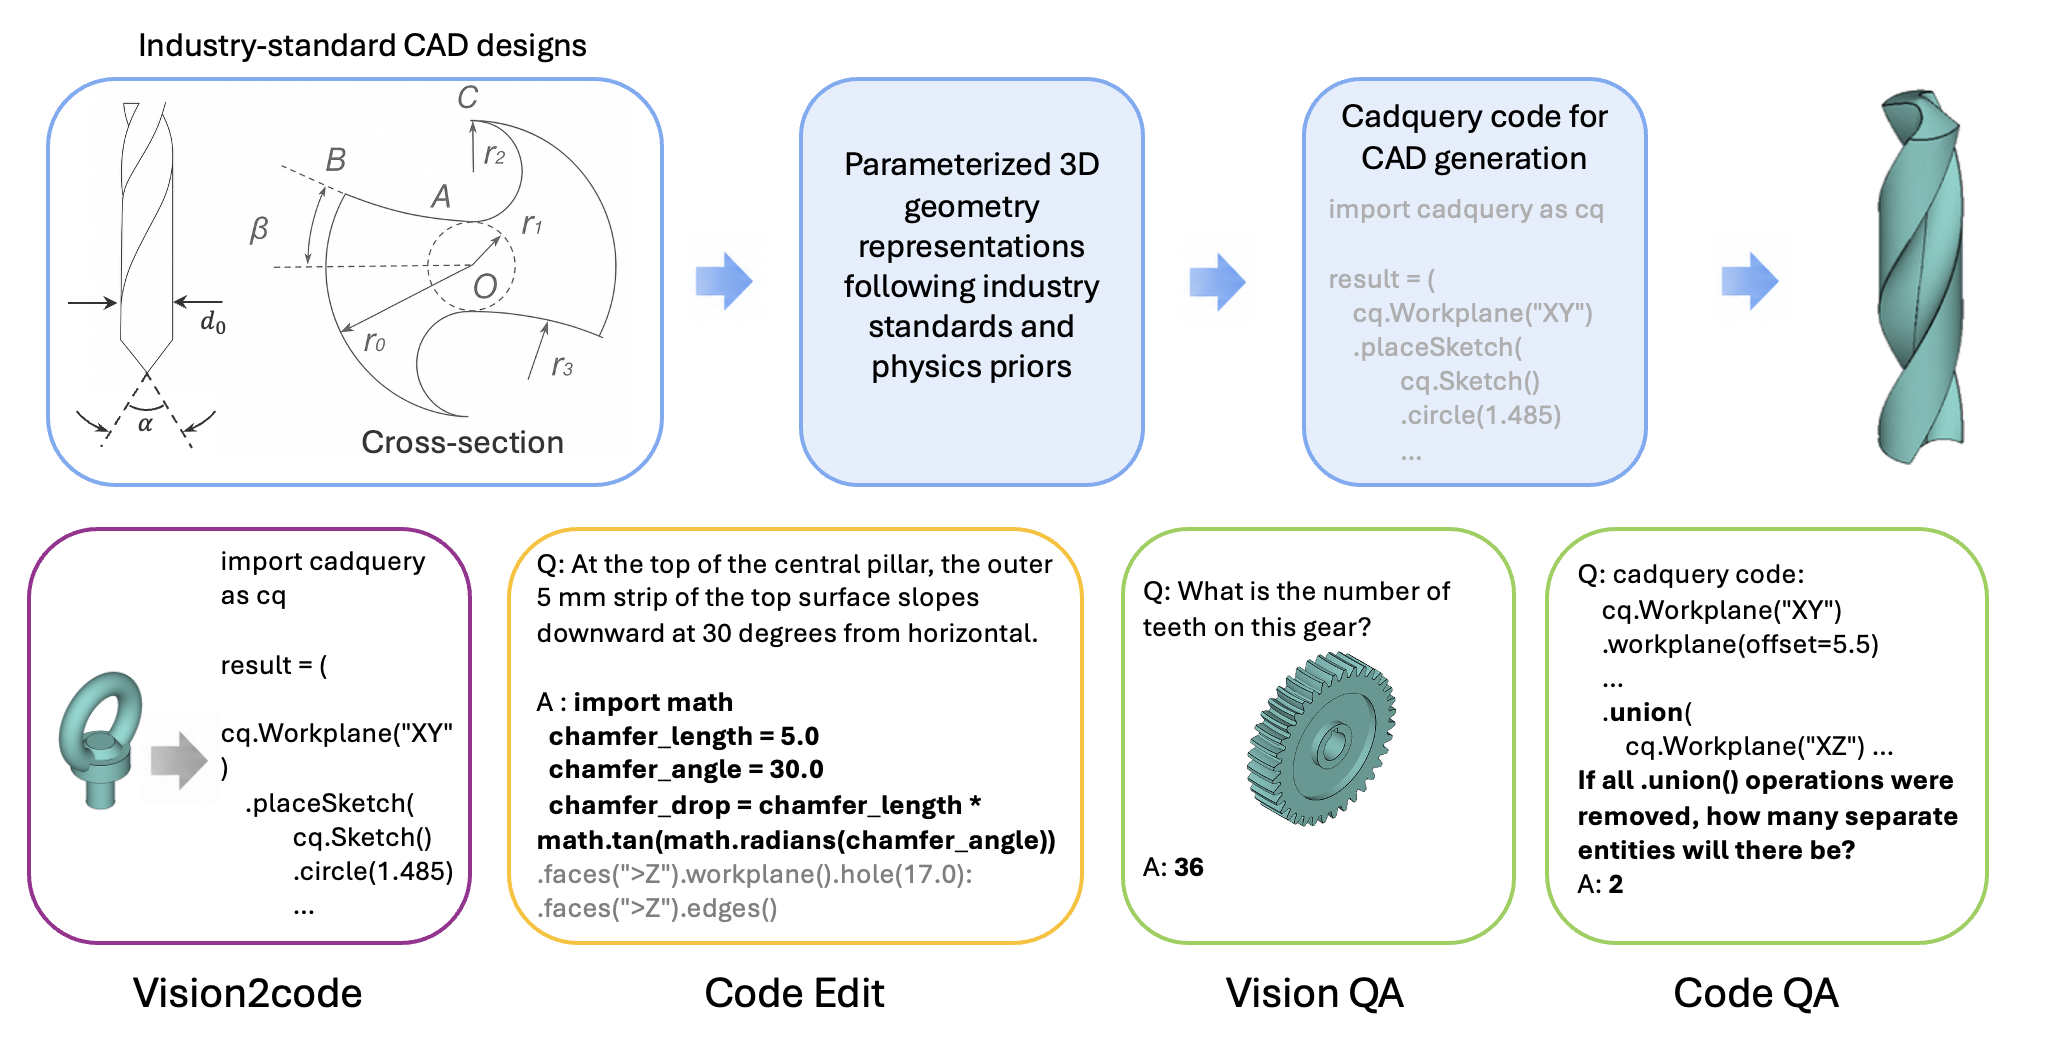
\includegraphics[width=\linewidth]{figures/fig_1.png}
  \caption{\textbf{BenchCAD overview.} \emph{Top:} BenchCAD parts originate from industry-standard engineering designs (e.g.\ DIN~338 twist drill cross-section), are realised as parameterised 3D geometry that respects the standard's parameter relations, and are emitted as executable CadQuery code. \emph{Bottom:} the four BenchCAD evaluation task categories: \texttt{img2cq} (image to CadQuery), \texttt{edit\_code} (instruction-guided code editing), \texttt{qa\_img} (visual numeric QA), and \texttt{qa\_code} (code-conditioned numeric QA).}
  \label{fig:teaser}
\end{figure}

Programmatic computer-aided design --- writing parametric scripts in CadQuery~\citep{CadQuerySoftware}, OpenSCAD, or Fusion's Python API that compile to manufacturable solid geometry --- has become the natural interface between large language models and the physical-design pipeline. A vision-language model (VLM) that reads an engineering drawing, emits executable CAD code, answers dimensional queries about that code, and revises its output to natural-language instructions would compress weeks of mechanical drafting into seconds, and several recent works have begun to deliver pieces of this promise~\citep{Khan2024,Guan2025,Rukhovich2025,Alrashedy2025,Kolodiazhnyi2026}. Yet a careful reader of these benchmarks notices an awkward pattern: the models that score highest on Chamfer distance often produce parts that \emph{look} correct in renders but fail every parametric query against the ground truth. When asked to reconstruct a DIN~338 twist drill (Figure~\ref{fig:teaser}, top) from four canonical views, a state-of-the-art reasoning model emits a CadQuery script whose helix angle, point angle, and flute geometry are all wrong by 8--22\%, yet the rendered solid is visually convincing enough to pass single-metric IoU evaluation. \textbf{The geometry passes the eye; it fails the calliper.}

This pattern is invisible to existing CAD code-generation benchmarks because they collapse three distinct capabilities into a single score. We propose to decompose the image-to-code pipeline into a three-rung \emph{parametric pyramid} for the purpose of benchmarking: at the base, \textbf{visual perception and 3D reconstruction}, where the model integrates four orthographic views into a coherent volumetric understanding; in the middle, \textbf{geometric-to-parametric abstraction}, where it identifies the parametric structure underlying that volume (which dimensions are bores, which are wall thicknesses, which are ratios fixed by industrial standards); and at the top, \textbf{parametric-to-code synthesis}, where it translates the parametric description into syntactically valid, executable CadQuery code. The decomposition is not a cognitive claim but a measurement scaffold: a single Chamfer-distance score collapses all three rungs and tells us that a model failed but not \emph{which rung gave way}. Prior CAD code-generation benchmarks reside near the base of this pyramid --- Text2CAD~\citep{Khan2024} supplies natural-language conditioning for sketch+extrude command sequences over DeepCAD~\citep{Wu2021}; CAD-Coder~\citep{Guan2025} applies SFT and GRPO with a Chamfer reward to produce CadQuery code from text; the CAD-Recode/cadrille/CADEvolve lineage~\citep{Rukhovich2025,Kolodiazhnyi2026,Elistratov2026} reverse-engineers point clouds and multi-view images into CadQuery via large procedural training corpora --- but none probe the middle rung directly, and none isolate the rungs from one another.

Three structural limitations compound this measurement gap. \textbf{While} prior CAD code-generation training corpora are dominated by sketch + extrude operations --- DeepCAD, Text2CAD, CAD-Recode, and cadrille contain essentially no helical sweeps, lofts, twist-extrudes, or parametric \emph{involute} gear-tooth construction; CADEvolve's recent evolutionary expansion broadens the seed pool to revolve, loft, sweep, fillet, chamfer, shell, and patterns but still lacks helical paths (used by coil springs, twist drills, and screw threads) and parametric involute-gear construction --- whereas industrial parts in the Fusion360 Gallery~\citep{Willis2021fusion} routinely compose 20+ distinct operations within a single component, including operations entirely absent from the prior corpora above (Appendix~\ref{app:ops}). \textbf{Conversely,} the benchmark with the broadest manual coverage, CADPrompt~\citep{Alrashedy2025}, contains only 200 expert-authored examples without family taxonomy, difficulty stratification, or scale-invariant prompts; its absolute-millimetre cues leak the answer to every ratio-based query that a properly designed numeric QA task would ask. \textbf{Furthermore,} ground truth across all four prior works is either parsed without re-execution (DeepCAD), filtered only by Chamfer threshold (CAD-Coder, CAD-Recode), or limited to a few hundred samples (CADPrompt) --- and none use a rotation-invariant IoU, so a geometrically correct but axis-permuted solid is silently penalised. Finally, no prior public CAD benchmark provides an instruction-guided code-editing task with execution-verified before/after pairs and a non-target preservation metric --- a gap that is especially consequential because editing differs structurally from generation: it requires \emph{locality} (changing only the targeted feature) and \emph{parameter-dependency reasoning} (preserving constraints that link the targeted feature to the rest of the program), neither of which can be measured by a generation metric on the edited output alone.

To address these gaps, we introduce \textbf{BenchCAD}, a CAD code-generation benchmark designed around three principles: industrial-standard anchoring, operation breadth, and capability decomposition. The dataset comprises 17{,}900 procedurally generated parts spanning 106 parametric families. Of these families, 49\% are bound to ISO, DIN, EN, ASME, or IEC specification tables --- DIN~338 twist drills, ISO~23509 bevel gears, DIN~2095 compression springs, DIN~8187 roller chains --- with parameters sampled from real specification ranges; the remaining 54 families cover bespoke industrial parts (twisted brackets, lobed knobs, mounting plates, custom impellers) governed by analogous proportional rules described in the released family code. The CadQuery operations exercised span 45+ distinct API calls including twist-extrusion, lofting, sweeping, helical sketches, and rectangular and polar patterns. Every record is execution-validated: the CadQuery source is re-run inside a sandbox, the resulting STEP voxelised at $64^3$ resolution, and matched against a reference solid by a 6-orientation rotation-invariant IoU $\geq 0.99$ before entering the verified split. Atop this dataset we define \textbf{five evaluation tasks across four categories} --- image-to-code (\texttt{img2cq}), image- and code-conditioned numeric QA (\texttt{qa\_img}, \texttt{qa\_code}), and image- and text-conditioned editing (\texttt{edit\_img}, \texttt{edit\_code}) --- in which two image/code pairs (\texttt{qa\_img}$\leftrightarrow$\texttt{qa\_code} and \texttt{edit\_img}$\leftrightarrow$\texttt{edit\_code}) form matched contrasts whose score \emph{difference} isolates which rung of the parametric pyramid is the bottleneck for a given model, while \texttt{img2cq} measures end-to-end generation.

Across our evaluation of 30+ frontier models, the diagnostic differential is striking. Even the strongest reasoning models --- GPT-5, Claude 4.6 Opus, o3 --- score 15--20 percentage points lower on image-conditioned numeric QA than on the matched code-conditioned variant; this gap survives chain-of-thought prompting, persists across the 1B-to-78B Qwen2.5-VL and InternVL3 scaling series, and is unchanged by supplying eight views instead of four. We name this systematic image-versus-code gap the \textbf{Vision Bottleneck} (\S\ref{sec:exp_capability}). On the editing task, 64\% of nominally successful edits exhibit \textbf{Edit Leakage} (\S\ref{sec:exp_edit}) --- the requested change is applied but unrelated parametric features are silently corrupted --- and multi-step edits requiring parameter-dependency reasoning collapse below 15\% pass rate. A matched-compute SFT ablation (\S\ref{sec:op_gap}; identical token count, optimiser, and seed across conditions) further reveals an \textbf{Op Vocabulary Gap}: models trained on sketch+extrude data alone achieve 0\% recall on every essential operation (helix, sweep, loft, twist-extrude, parametric involute-gear construction), and recover only after 81K BenchCAD samples replace half the training mix (per-op breakdown in \S\ref{sec:op_gap}). Together these findings suggest that the path forward lies in training procedures explicitly aware of the parametric-symbolic structure of CAD geometry, rather than continued scaling of code-finetuned VLMs.

\paragraph{Our contributions are threefold.}
\begin{enumerate}[leftmargin=1.4em,topsep=4pt,itemsep=4pt]
  \item \textbf{The BenchCAD dataset and CadGen pipeline.} We release 17{,}900 verified parametric CAD parts spanning 106 families (49\% anchored to ISO/DIN/EN/ASME/IEC specification tables), exercising 45+ distinct CadQuery operations, supplemented by a 2{,}400-question paired numeric QA bank, a 748-pair instruction-guided edit subset, a 530-sample stratified Lite split for rapid leaderboards, and a 162{,}000-pair training corpus derived from GenCAD~\citep{GenCAD2025}. Underlying the dataset is CadGen, a procedural construction pipeline integrating standard-table sampling, op-list emission, sandboxed execution under a $64^3$ rotation-invariant 3D IoU $\geq 0.99$ verification, and Croissant 1.0 metadata~\citep{Croissant2024}; all releases are publicly hosted under \texttt{BenchCAD/cad\_bench} on Hugging Face under CC-BY-4.0.
  \item \textbf{A capability-decomposed benchmark with the first verified parametric edit task.} We define five evaluation tasks --- \texttt{img2cq}, \texttt{qa\_img}, \texttt{qa\_code}, \texttt{edit\_img}, \texttt{edit\_code} --- where two image/code pairs (\texttt{qa\_img}$\leftrightarrow$\texttt{qa\_code} and \texttt{edit\_img}$\leftrightarrow$\texttt{edit\_code}) form matched contrasts whose score difference directly isolates which rung of the parametric pyramid is the bottleneck. To our knowledge, BenchCAD-Edit is the first publicly released CAD benchmark combining execution-verified before/after CadQuery code pairs with a non-target preservation metric distinguishing target-feature \emph{success} from program-wide \emph{locality}.
  \item \textbf{Three diagnostic phenomena: Vision Bottleneck, Edit Leakage, and Op Vocabulary Gap.} Across 30+ frontier vision-language and code-language models we identify three systematic phenomena: (i) a 15--20 point gap between code- and image-conditioned numeric QA (the \emph{Vision Bottleneck}), surviving chain-of-thought prompting, parameter scaling from 1B to 78B, and view-count augmentation; (ii) a 64\% \emph{Edit Leakage} rate on nominally successful edits where unrelated parametric features are silently corrupted; and (iii) an \emph{Op Vocabulary Gap} where matched-compute SFT on sketch+extrude data alone yields zero recall on essential operations until BenchCAD-Synth enters the training mix. These findings refocus the CAD-LM research agenda from code-synthesis improvements toward visual-to-parametric reconstruction, parameter-dependency reasoning, and operation-coverage in training corpora.
\end{enumerate}

\section{Related Work}
\label{sec:related}

\paragraph{Command-sequence CAD generation.}
The first wave of programmatic CAD generation operates on \emph{command-sequence representations} of sketch-and-extrude operations. DeepCAD~\citep{Wu2021} introduces a 178K-model corpus of Onshape parts encoded as discrete operation tokens, and Text2CAD~\citep{Khan2024} extends DeepCAD with 660K natural-language annotations spanning four abstraction levels, training a BERT-conditioned autoregressive transformer to emit those tokens. CAD-Coder~\citep{Guan2025} reformulates the same underlying data as CadQuery Python source and applies SFT + GRPO with a chain-of-thought prefix and Chamfer-distance reward, reaching mean CD $6.54\!\times\!10^{-3}$ on the Text2CAD test split.

\paragraph{The CadQuery-VLM lineage.}
A parallel research program has driven the recent state of the art in CadQuery code generation through three iterative releases. CAD-Recode~\citep{Rukhovich2025} first established the CadQuery formulation for reverse engineering, fine-tuning a Qwen2-1.5B language model on a procedurally generated corpus of 1M sketch-and-extrude scripts and reporting mean Chamfer distance 0.30 and IoU 92.0 on DeepCAD. cadrille~\citep{Kolodiazhnyi2026} extends this base by upgrading to Qwen2-VL-2B and unifying point-cloud, multi-view image, and text inputs in a single model, then introducing online reinforcement learning via Dr.CPPO with a piecewise IoU reward; the resulting cadrille-RL reaches DeepCAD image IoU 92.2 and Fusion360 image IoU 84.6 with 0.0\% invalidity. CADEvolve~\citep{Elistratov2026} shares the same backbone and RL recipe but expands the training corpus to 2.7M scripts via an LLM-driven evolutionary loop whose seed pool covers extrude, revolve, loft, sweep, fillet, chamfer, shell, Boolean operations, and patterns --- significantly broadening the operation distribution while still lacking helical sweeps and parametric involute-gear construction --- and achieves DeepCAD image IoU 92.6. All three release model weights and inference scripts under permissive licences; we evaluate the latter two on BenchCAD as transfer baselines (\S\ref{sec:transfer}). These works collectively demonstrate the viability of CadQuery as a generation target and establish $\sim$92\% IoU as the saturated ceiling on existing benchmarks. They share three structural limitations BenchCAD addresses: \textit{(i)} training and evaluation data remain dominated by sketch+extrude --- CAD-Recode/cadrille restrict to sketch+extrude+Boolean while CADEvolve's broader seed pool still omits helical sweeps and parametric involute-gear construction; \textit{(ii)} evaluation lacks both family-level taxonomy and standard-table grounding; and \textit{(iii)} none decouple sub-capabilities --- every prior benchmark scores a single end-to-end metric, conflating visual perception, geometric abstraction, and code synthesis.

\paragraph{CAD code-generation and editing benchmarks.}
CADCodeVerify~\citep{Alrashedy2025} introduces \textbf{CADPrompt}, the first quantitative CAD code-generation benchmark --- 200 natural-language prompts paired with expert CadQuery code, scored via point-cloud distance and bounding-box IoU after ICP alignment. Despite establishing a useful protocol, CADPrompt is two orders of magnitude smaller than BenchCAD's verified split (17{,}900), lacks family taxonomy or difficulty stratification, leaks scale via absolute millimetre cues in prompts, and uses axis-aligned IoU that penalises geometrically correct but axis-permuted solutions. Two concurrent editing-focused works leave complementary gaps: CAD-Editor~\citep{CADEditor2025} proposes a locate-then-infill pipeline trained entirely on synthetic edit data without releasing a held-out human-verified edit benchmark, and CADialogue~\citep{CADialogue2025} evaluates ten edit tasks within a conversational interface but does not release the eval set publicly. HistCAD~\citep{Dong2026} measures the preservation of ten geometric-constraint types under edits via a FreeCAD edit-then-check protocol, but operates at the sketch-constraint level rather than at the executable-program level. To our knowledge, BenchCAD-Edit is the first publicly released CAD benchmark to combine: (i) execution-verified before/after CadQuery code pairs, (ii) a non-target preservation metric distinguishing target-feature success from program-wide locality, and (iii) cross-family balanced coverage with explicit edit-category taxonomy.

\paragraph{Position of BenchCAD.}
We borrow three structural patterns from recent benchmark methodology in adjacent domains: explicit task taxonomy with per-task representative items (MMSI-Bench~\citep{MMSIBench2026}), Lite + Full split design for differentiated evaluation cost (AutoCodeBench~\citep{Chou2026}), and a small set of named, quantitative findings as the paper's punch line (Infinity-Chat~\citep{Hivemind2025}). Within CAD code generation specifically, BenchCAD is the first benchmark to combine four properties simultaneously: (i) \emph{execution-verified at scale} (17{,}900 parts at IoU $\geq 0.99$), (ii) \emph{standard-anchored} (49\% of families bound to ISO/DIN/EN/ASME/IEC specification tables), (iii) \emph{operation-rich} (45+ CadQuery operations versus 2--5 in prior corpora), and (iv) \emph{capability-decomposed} (five tasks with two image/code matched-contrast pairs that isolate visual reconstruction, parametric abstraction, and code synthesis along the image$\to$code causal chain, including the first verified parametric edit task). Table~\ref{tab:cmp_prior} summarises this comparison.

\begin{table*}[t]
\centering
\small
\setlength{\tabcolsep}{3pt}
\caption{\textbf{BenchCAD versus prior CAD code-generation benchmarks.} To our knowledge, BenchCAD is the first public CAD benchmark to simultaneously offer an industrial part-family taxonomy, parameter anchoring against ISO/DIN/EN/ASME/IEC specification tables at scale, and operation coverage that includes all four advanced operation families. \textbf{Columns:} \textbf{\#Indus.\ fam.} = number of \emph{named} industrial part families with explicit functional identity (gear, drill, spring, $\ldots$), versus untyped CAD parts pooled without semantic structure; \textbf{\#Std codes} = number of distinct ISO/DIN/EN/ASME/IEC specification codes from which parameter ranges are programmatically sampled; \textbf{\#Distinct CQ ops} = number of distinct CadQuery API operations exercised across the released dataset (counts derived from each work's published description; ours from a static analysis of the released family code, see Appendix~\ref{app:ops}); \textbf{Adv ops} = whether the dataset exercises \emph{all four} advanced operation families: helix (helical sweeps), loft/sweep, twist-extrude, and parametric involute-gear construction. -- denotes absence relative to the column's definition rather than an exhaustive file-level audit. \cmark$\,$ = supported, part.\, = partial, -- = absent.}
\label{tab:cmp_prior}
\begin{tabular}{lrrrrlcccccc}
\toprule
                                    &      & \#Sam-  & \#Indus.\ & \#Std  & \#Distinct                & Adv  &        &        & Scale & Edit & QA \\
Benchmark                           & Year & ples    & fam.      & codes  & CQ ops                    & ops  & Verif. & RotIoU & inv.  & task & task \\
\midrule
DeepCAD~\citep{Wu2021}              & '21 & 178K   & 0    & 0   & 4 (sk+ex)                       & --     & --     & --     & --     & --     & --     \\
Fusion360 G.~\citep{Willis2021fusion} & '21 & 8K   & 0    & 0   & $\sim$6 (sk+ex+rev+fil)         & --     & --     & --     & --     & --     & --     \\
Text2CAD~\citep{Khan2024}           & '24 & 170K   & 0    & 0   & 4 (sk+ex)                       & --     & --     & --     & --     & --     & --     \\
CADPrompt~\citep{Alrashedy2025}     & '25 & 200    & 0    & 0   & varied (manual)                 & part.  & part.  & --     & --     & --     & --     \\
CAD-Coder~\citep{Guan2025}          & '25 & 110K   & 0    & 0   & 4 (sk+ex)                       & --     & \cmark & --     & --     & part.  & --     \\
CAD-Recode~\citep{Rukhovich2025}    & '25 & 1M+7K  & 0    & 0   & 6 (sk+ex+bool)                  & --     & \cmark & --     & --     & part.  & seq.   \\
cadrille~\citep{Kolodiazhnyi2026}   & '26 & 1M+7K  & 0    & 0   & 6 (sk+ex+bool)                  & --     & \cmark & --     & --     & --     & --     \\
CADEvolve~\citep{Elistratov2026}    & '26 & 2.7M   & 0    & 0   & $\sim$12 (+rev,\,loft,\,sweep,\,fil,\,cham,\,sh)\textsuperscript{*} & part.\textsuperscript{*} & \cmark & --     & --     & --     & --     \\
\midrule
\textbf{BenchCAD (ours)} & \textbf{'26} & \textbf{17{,}900} & \textbf{106} & \textbf{47} & \textbf{45+} & \textbf{\cmark} & \textbf{\cmark} & \textbf{\cmark} & \textbf{\cmark} & \textbf{\cmark} & \textbf{\cmark} \\
\bottomrule
\end{tabular}

\vspace{2pt}
{\footnotesize\textsuperscript{*}CADEvolve's seed pool covers extrude, revolve, loft, sweep, shell, fillet, chamfer, Boolean operations, and patterns, exercising 2 of the 4 advanced families (loft/sweep). The remaining two advanced families --- helical sweeps (used by coil springs, twist drills, screw threads) and parametric involute-gear construction --- remain absent from the released training corpus.}
\end{table*}


\section{The BenchCAD Dataset}
\label{sec:dataset}

\subsection{Design Principles}
We design BenchCAD around four principles that prior CAD datasets violate either individually or jointly.

\paragraph{P1 --- Execution as ground truth.} Every record's ground truth is the \emph{executed} solid: the CadQuery source code is run inside a sandboxed CadQuery / PythonOCC environment, the resulting STEP file is voxelised, and compared against a reference solid by 3D IoU under the rotation-invariant 6-face cube group~\citep{rot_iou}. A record enters the verified split only if IoU $\geq 0.99$ \emph{and} executes within a 30\,s timeout with non-degenerate volume. This rules out the silent failure mode common in DeepCAD-derived corpora where parsed code is assumed correct but neither re-executed nor geometrically validated.

\paragraph{P2 --- Standard-table anchoring.} Where a part has an industrial counterpart, parameters sample from real specification tables (ISO 22 V-belt cross-section series, DIN 338 twist-drill diameter ranges, ISO 23509 bevel-gear pitch--module relationship). Geometry that ``looks right'' but violates manufacturable proportions (e.g.\ M6 bolt with 3\,mm thread pitch) is rejected at sampling time. 49\% of BenchCAD families (52/106) are standard-anchored, drawing from 47 unique ISO/DIN/EN/ASME/IEC codes; Table~\ref{tab:standards} enumerates the breakdown.

\paragraph{P3 --- Family-level taxonomy.} Records are grouped into 106 named families (e.g.\ \texttt{coil\_spring}, \texttt{helical\_gear}, \texttt{twisted\_drill}), each implemented by a small Python module exposing a typed parameter schema, a sampler, a validator, and a deterministic builder. This makes coverage measurable, sampling reproducible, difficulty controllable, and per-family analysis trivial --- properties absent from DeepCAD/Fusion360 where parts are pooled without semantic structure.

\paragraph{P4 --- Operation breadth.} The dataset exercises 45+ distinct CadQuery operations spanning sketch primitives, contour drawing (lines, arcs, splines), workplane manipulation, sketch arrays, 3D operations (extrude, twist-extrude, revolve, loft, sweep), Booleans, hole variants, and edge finishing (fillet, chamfer, shell). Appendix~\ref{app:ops} contrasts this against prior corpora restricted to sketch+extrude.

\subsection{Family Registry and Standard Compliance}
Each family is a class implementing the \texttt{Family} interface: a JSON-schema parameter spec; a \texttt{sample\_params(difficulty, rng)} method that draws a parameter dictionary; a \texttt{validate\_params(p)} predicate enforcing geometric and standard-table constraints; and a \texttt{make\_program(p)} method that emits a typed list of \texttt{Op} dicts consumable by the builder. Families are auto-discovered from a registry module; adding a new family requires no changes to the pipeline beyond registering one class. A family declares \texttt{standard = "ISO 23509"} (etc.) when its parameter ranges and inter-parameter relations are fixed by an external specification table. As of submission, BenchCAD covers 17 ISO codes (e.g.\ ISO 22, 53, 113, 272, 606, 1234, 2339, 2936, 5167-4, 10828, 23509), 21 DIN codes (e.g.\ DIN 338, 471/472, 580, 5480, 2095, 8187, 71412), 4 EN codes (10034, 10056, 10219, 10279), 3 ASME codes (B1.20.1, B16.5, B16.9), and 2 IEC codes (60072-1, 60086) --- 47 unique codes across 52 standard-anchored families. The remaining 54 families cover bespoke industrial parts (e.g.\ \texttt{twisted\_bracket}, \texttt{venturi\_tube}, \texttt{lobed\_knob}) without formal standards but governed by analogous proportional rules.

Each family supports three difficulty tiers --- \emph{easy}, \emph{medium}, \emph{hard} --- defined by parameter complexity (op count, feature count, non-axis-aligned geometry, presence of helical, lofted, or boolean operations). Tier definitions are family-specific and machine-checkable; aggregate counts appear in Table~\ref{tab:family_cliff}.

\begin{table}[t]
\centering
\small
\caption{\textbf{Standard-anchored families.} 49\% of BenchCAD families (52/106) bind their parameters to ISO/DIN/EN/ASME/IEC specification tables, sampling at values drawn from real engineering ranges rather than arbitrary geometry. The bottom row counts the 54 custom families covering bespoke industrial parts (twisted brackets, lobed knobs, etc.) governed by analogous proportional rules without formal standards.}
\label{tab:standards}
\begin{tabular}{llrr}
\toprule
Standard & Codes covered (sample) & \#Codes & \#Fam. \\
\midrule
ISO   & 22, 53, 113, 272, 606, 1234, 2339, 2936, 5167-4, 10828, 23509, \ldots & 17 & 18 \\
DIN   & 315, 338, 471/472, 580, 660, 705, 950, 988, 2095, 5480, 6885, 8187, 71412, \ldots & 21 & 21 \\
EN    & 10034, 10056, 10219, 10279                       & 4 & 5 \\
ASME  & B1.20.1, B16.5, B16.9                            & 3 & 5 \\
IEC   & 60072-1, 60086                                   & 2 & 2 \\
\midrule
\textbf{Total standard-anchored}   & & \textbf{47} & \textbf{52 (49\%)} \\
Custom (no formal standard)        & & --          & 54 \\
\bottomrule
\end{tabular}
\end{table}


\subsection{The CadGen Pipeline}
We name the data construction pipeline \textbf{CadGen} to separate it as a standalone contribution from the resulting dataset. CadGen has four stages.

\paragraph{Stage 1 --- Parameter sampling.} For each family $\times$ difficulty bucket, the sampler draws parameters from the JSON schema under standard-table constraints. Sampling is deterministic given a seed.

\paragraph{Stage 2 --- Program emission.} The family's \texttt{make\_program} returns an op sequence. The builder consumes the op list and produces (i) Python CadQuery source code via a per-op code template, and (ii) a CadQuery \texttt{Workplane} object via direct API dispatch. Both representations are aligned by construction: the same op list yields equivalent geometry whether interpreted via the builder or by executing the emitted code in a fresh sandbox.

\paragraph{Stage 3 --- Execution and verification.} We re-execute the emitted code in an isolated sandbox, export STEP, voxelise at 64$^3$ resolution, and compute rotation-invariant 3D IoU against the builder's direct STEP output. Records with IoU $< 0.99$, execution failures, timeouts ($>$30\,s), or zero/inverted volume are quarantined for review. A persistent execution cache avoids re-running the same code on subsequent syncs.

\paragraph{Stage 4 --- Render and package.} Each verified record is rendered to four canonical views (front / right / top / iso) at 512$\times$512 with VTK, and the (parameters, program, code, STEP, views) bundle is registered to the dataset CSV.

\paragraph{Yield.} From a 17{,}968-sample run on the April 2026 batch, 17{,}900 records (99.6\%) passed all checks; the 78 failures concentrated in three pathological families (\texttt{double\_simplex\_sprocket}, \texttt{stepped\_shaft}, \texttt{torus\_link}) due to OCCT \texttt{Standard\_Failure} on extreme parameter combinations.

\subsection{Splits, Documentation, and Hosting}
\paragraph{Splits.} The full release contains six subsets (Table~\ref{tab:dataset}): \emph{BenchCAD-Synth} (17{,}900 verified procedural parts, primary evaluation set); \emph{BenchCAD-Edit} (748 curated edit pairs spanning dimensional / additive / subtractive / multi-step modifications across 106 families); \emph{BenchCAD-Lite} (530-sample stratified subset for fast leaderboards); \emph{BenchCAD-Fusion360} and \emph{BenchCAD-DeepCAD} (verified subsets for OOD evaluation); and \emph{BenchCAD-GenCAD} (162{,}000 image-to-code pairs derived from GenCAD~\citep{GenCAD2025} for SFT-scale training).

\paragraph{Documentation, hosting, licence.} Every dataset ships with a Croissant 1.0 metadata file~\citep{Croissant2024} including all required Responsible AI fields. Validation passes the public Croissant checker. All splits are hosted on Hugging Face under \texttt{BenchCAD/cad\_bench} (test) and \texttt{BenchCAD/cad\_bench\_edit} (edit), with the verification-pipeline source under MIT and the dataset under CC-BY-4.0. Dataset cards link to per-family parameter schemas and the standard-table sources used for compliance. A datasheet following~\citet{rot_iou} appears in Appendix~\ref{app:datasheet}.

\begin{table}[t]
\centering
\small
\caption{\textbf{BenchCAD dataset composition.} The verified evaluation core consists of 17{,}900 procedurally generated parts spanning 106 families, with each record carrying parametric source code, executable STEP, four canonical-view renders, and a parameter JSON. The QA bank contains 2{,}400 paired questions evaluated under both visual and code conditioning. We additionally release an Edit subset, a stratified Lite split, two OOD subsets, and a 162K-pair training corpus.}
\label{tab:dataset}
\begin{tabular}{lrrl}
\toprule
Split & \#Records & \#Families & GT artefacts \\
\midrule
BenchCAD-Synth (verified)    & 17{,}900 & 106 & code $\cdot$ STEP $\cdot$ 4 views $\cdot$ params $\cdot$ ops \\
BenchCAD-QA (paired img/code)& 2{,}400 $\times 2$ & 106 & question $+$ gold answer \\
BenchCAD-Edit                & 748      & 106 & before/after $+$ NL instruction \\
BenchCAD-Lite (stratified)   & 530      & 106 & same as Synth \\
BenchCAD-Fusion360 (verif.)  & 726      & 52  & + raw STEP \\
BenchCAD-DeepCAD (verif.)    & 920      & --  & code $\cdot$ STEP $\cdot$ views \\
\midrule
BenchCAD-GenCAD (training)   & 162{,}000 & -- & image $\cdot$ code (SFT pairs) \\
\bottomrule
\end{tabular}
\end{table}


\begin{figure}[t]
  \centering
  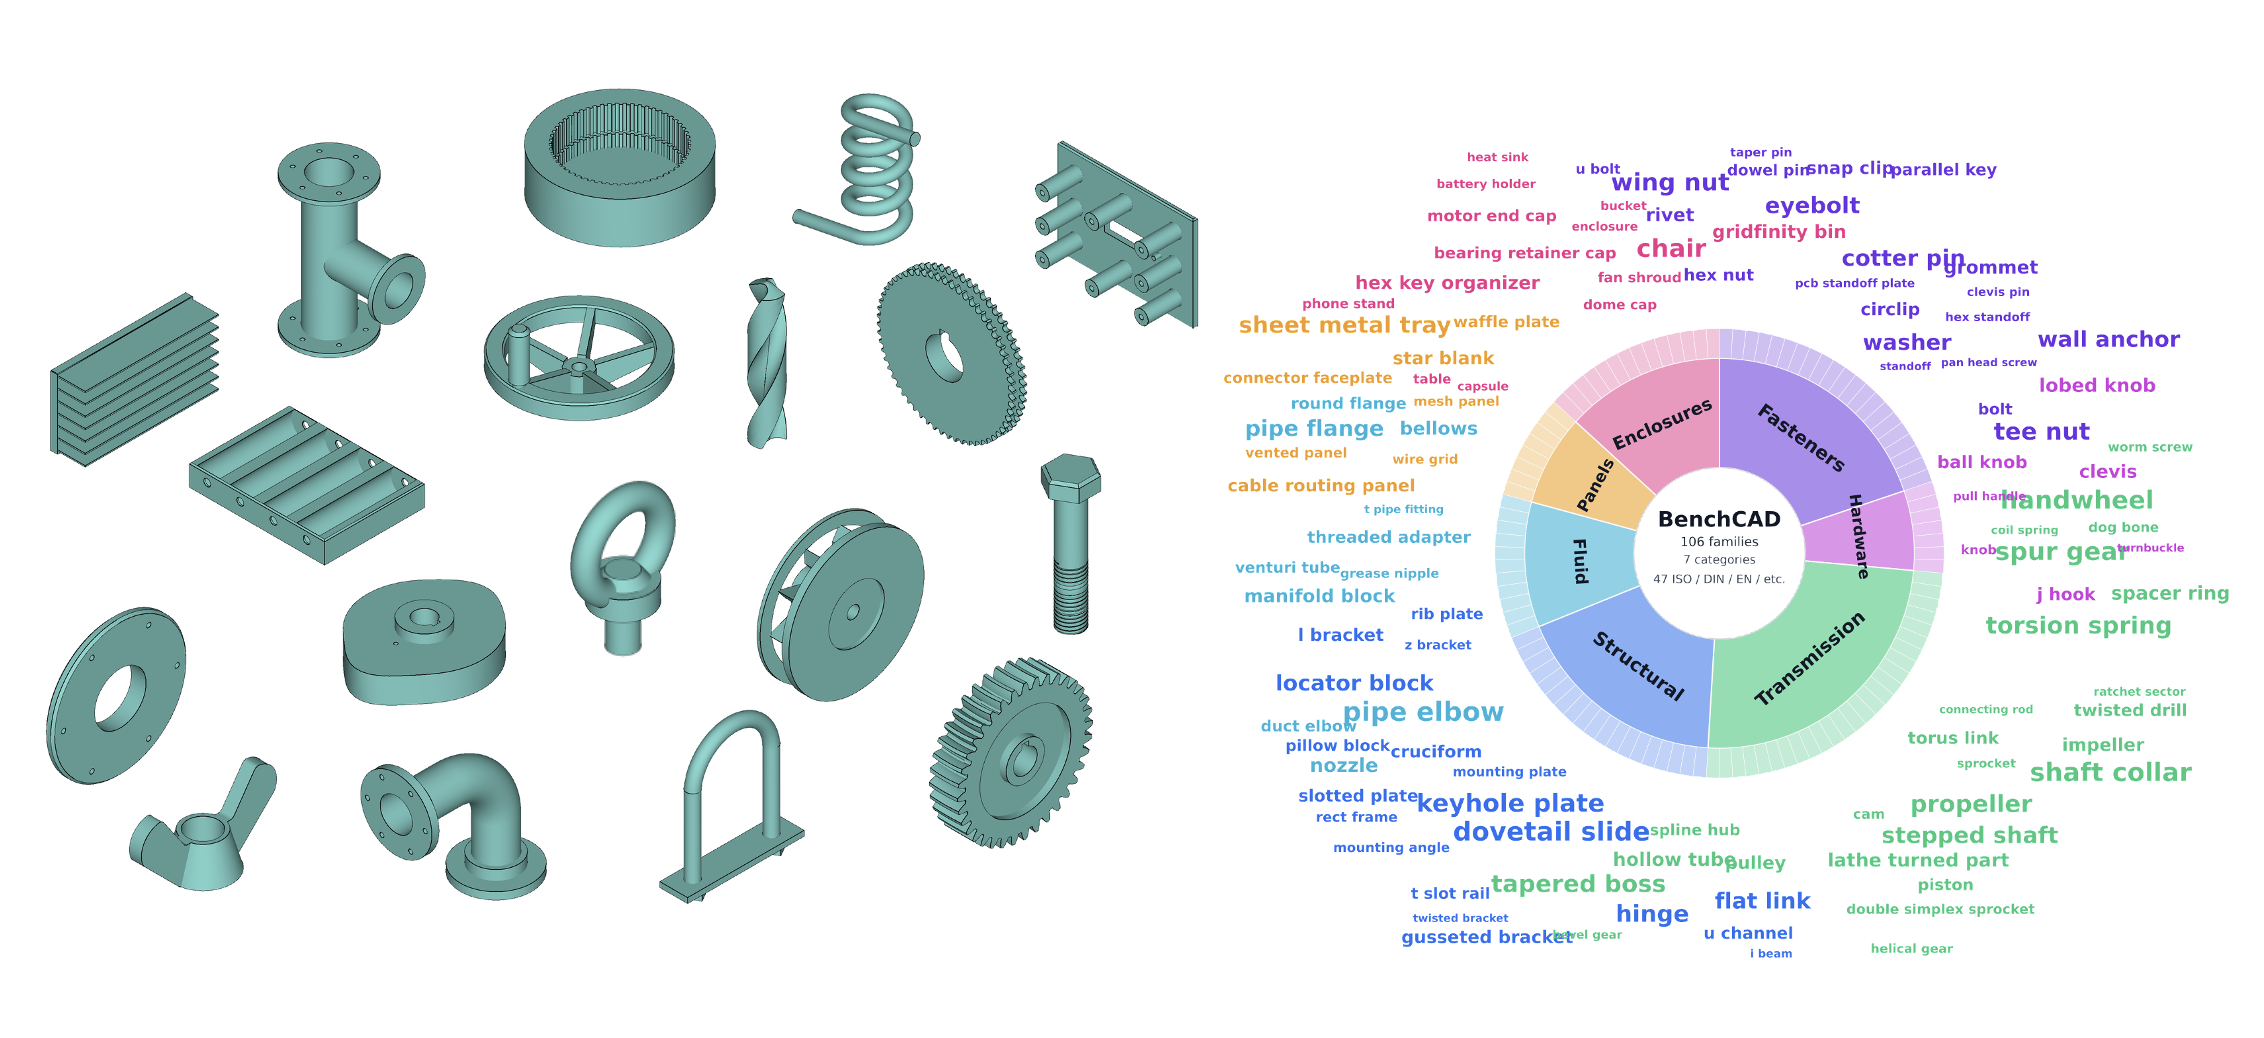
\includegraphics[width=\linewidth]{figures/fig_2.png}
  \caption{\textbf{BenchCAD dataset composition.} \emph{Left:} representative renders sampled across the 106 families, spanning fasteners (bolts, eye bolts, wing nuts), transmission components (spur gears, propellers, sprockets), structural elements (brackets, slotted plates, I-/U-channels), fluid fittings (pipe elbows, flanges), panels, hardware, and enclosures. \emph{Right:} the 106 families organised by seven functional categories (Fasteners / Hardware / Transmission / Structural / Fluid / Panels / Enclosures); 52 of the 106 families (49\%) are anchored to a named ISO / DIN / EN / ASME / IEC standard.}
  \label{fig:dataset_overview}
\end{figure}

\section{Benchmark Tasks and Capability Decomposition}
\label{sec:tasks}

\subsection{The Image$\to$Code Capability Chain}
\label{sec:capability}

A single end-to-end metric (Chamfer distance, IoU, pass rate) on an image-to-code task reports \emph{whether} a model succeeded, but not \emph{which capability} failed. Prior CAD code-generation benchmarks (Text2CAD, CAD-Coder, CAD-Recode, CADCodeVerify) score one such metric per model and conflate three distinct sub-capabilities required to map a multi-view image to executable parametric source.

We decompose the image$\to$code task into three causal links (Table~\ref{tab:capability}):
\begin{itemize}[leftmargin=1.2em,topsep=2pt,itemsep=2pt]
\item $C_1$ \textbf{Visual + 3D Reconstruction} ($f_{C_1}\!:\,\text{multi-view image} \to \text{3D shape}$). The model integrates four orthographic views into a coherent volumetric understanding.
\item $C_2$ \textbf{Geometric$\to$Parametric Abstraction} ($f_{C_2}\!:\,\text{3D shape} \to \{(p_i,v_i)\}$). The model identifies the parametric structure underlying the geometry: which dimensions are bores, which are wall thicknesses, which are ratios.
\item $C_3$ \textbf{Parametric$\to$Code Synthesis} ($f_{C_3}\!:\,\{(p_i,v_i)\} \to \text{CadQuery code}$). The model emits syntactically valid, executable code that realises the parameters in the target API (workplane choice, op order, fillet radii, hole alignment).
\end{itemize}

BenchCAD's five tasks are designed so that each task exercises a known subset of $\{C_1, C_2, C_3\}$, and so that score \emph{differences} across tasks isolate which capability is the bottleneck. The gap between \texttt{qa\_img} and \texttt{qa\_code} scores under matched prompts measures the cost of replacing direct code access with visual perception --- i.e.\ $C_1$ alone. We refer to this systematic gap as the \textbf{Vision Bottleneck}, and it is the central diagnostic finding of BenchCAD (\S\ref{sec:exp_capability}).

\paragraph{Diagnostic differentials.} Given a model's per-task scores, four interpretable contrasts apply:
\begin{itemize}[leftmargin=1.2em,topsep=2pt,itemsep=1pt]
\item \texttt{qa\_img} $-$ \texttt{qa\_code} (large negative) $\Rightarrow$ \emph{$C_1$ is the bottleneck}.
\item \texttt{qa\_code} (low absolute) $\Rightarrow$ \emph{$C_2$ is the bottleneck}.
\item \texttt{img2cq} $-$ \texttt{edit\_code} (large negative) $\Rightarrow$ \emph{$C_3$ + full-stack composition is the bottleneck}.
\item \texttt{edit\_img} $-$ \texttt{edit\_code} (large negative) $\Rightarrow$ Vision Bottleneck preserved on edit tasks.
\end{itemize}

\begin{table}[t]
\centering
\small
\caption{\textbf{Capability decomposition.} BenchCAD's five tasks isolate the three sub-capabilities along the image$\to$code causal chain: $C_1$ visual + 3D reconstruction, $C_2$ geometric$\to$parametric abstraction, and $C_3$ parametric$\to$code synthesis. Score differences across paired tasks (e.g.\ \texttt{qa\_img}$-$\texttt{qa\_code}) directly diagnose which capability is the bottleneck. ``part.'' indicates partial coverage (the original code constrains, but does not eliminate, the corresponding sub-capability).}
\label{tab:capability}
\begin{tabular}{llccc}
\toprule
Task & Input $\to$ Output & $C_1$ vision & $C_2$ param. & $C_3$ code \\
\midrule
\texttt{img2cq}    & 4 views $\to$ code              & \cmark & \cmark & \cmark \\
\texttt{qa\_img}   & 4 views $+$ Q $\to$ number      & \cmark & \cmark & --     \\
\texttt{qa\_code}  & code $+$ Q $\to$ number         & --     & \cmark & --     \\
\texttt{edit\_img} & views $+$ code $+$ instr $\to$ code  & \cmark & part.  & \cmark \\
\texttt{edit\_code}& code $+$ instr $\to$ code       & --     & part.  & \cmark \\
\bottomrule
\end{tabular}
\end{table}


\subsection{Task Definitions and Scoring}

\paragraph{Task 1 --- \texttt{img2cq} (image-to-code).} \emph{Inputs:} four canonical orthographic views (front / right / top / iso) of a verified part, plus a fixed system prompt requesting CadQuery source. \emph{Output:} CadQuery Python code. \emph{Score:} we re-execute the generated code, voxelise the resulting STEP, and compute rotation-invariant 3D IoU against the reference solid. The headline metric is $\mathrm{Pass}_{\mathrm{IoU}\geq 0.5}$, the fraction of generations achieving IoU $\geq 0.5$ under the cube symmetry group; we additionally report mean Chamfer distance, invalidity ratio (execution-failure rate), and Feature-F1 over primitive types.

\paragraph{Task 2 --- \texttt{qa\_img} (visual numeric QA).} \emph{Inputs:} the four views plus a numeric question (e.g.\ ``what is the ratio of inner to outer diameter?'', ``how many spokes does the wheel have?''). The BenchCAD-QA bank contains 2{,}400 unique questions sampled from a per-family template set that asks only ratios and integer counts --- never absolute lengths in millimetres --- making them invariant to overall part scale (\S\ref{sec:scoring}). \emph{Output:} a single number. \emph{Score:} relative error $\leq 5\%$ for ratios; exact match for integers. Question bank construction is in Appendix~\ref{app:qbank}.

\paragraph{Task 3 --- \texttt{qa\_code} (code-only numeric QA).} \emph{Inputs:} the same 2{,}400 numeric questions as \texttt{qa\_img}, but conditioned on the verified CadQuery source code instead of images. The paired design (each question evaluated under both modalities) directly isolates $C_2$ (parametric reasoning) from $C_1$ (visual perception); the model has perfect access to the underlying parameters and must derive the answer symbolically. \emph{Output and score:} same as \texttt{qa\_img}.

\paragraph{Task 4 --- \texttt{edit\_img} (image-conditioned edit).} \emph{Inputs:} the four views of an original part, the original CadQuery source, and a natural-language edit instruction (\emph{``add a 3\,mm chamfer on the outer top edges''}, \emph{``remove one of the four legs''}, \emph{``increase the bore diameter while keeping the tooth count''}). The BenchCAD-Edit split provides 748 curated instruction--edit pairs across 106 families, spanning four categories (dimensional, additive, subtractive, multi-step). \emph{Output:} edited code. \emph{Score:} Pass@1 = $\mathbb{1}[\mathrm{IoU}(\text{edited}, \text{target}) \geq 0.99 \wedge \mathrm{Preserve}(\text{edited}, \text{orig}) \geq 0.99]$, requiring \emph{both} target success \emph{and} non-target preservation; we additionally report the disaggregated Edit Leakage rate (\S\ref{sec:exp_edit}).

\paragraph{Task 5 --- \texttt{edit\_code} (text-only edit).} \emph{Inputs:} same as \texttt{edit\_img} but without the images. This is the text-only counterpart of \texttt{edit\_img} and isolates $C_3$ (code synthesis under natural-language guidance) without visual context. \emph{Output and score:} as \texttt{edit\_img}. To our knowledge BenchCAD-Edit is the first public benchmark targeting instruction-guided CAD code editing as a first-class evaluation with execution-verified before/after pairs and a non-target preservation metric.

\paragraph{Aggregate.} The headline aggregate is the macro-mean across the five tasks (\emph{Avg}). We report per-difficulty splits in Table~\ref{tab:family_cliff}.

\subsection{Invariance and Honesty in Scoring}
\label{sec:scoring}
Two design choices distinguish BenchCAD's scoring from prior practice.

\paragraph{Rotation invariance.} A solid that is geometrically correct but axis-permuted is correct from a manufacturing standpoint --- the user can re-install the workpiece in any of the cube symmetries. We compute IoU as the maximum over the 6 face-up orientations (or the full 24-element cube rotation group, configurable at evaluation time) instead of single-axis-aligned IoU. This avoids the systematic underestimation observed in CADPrompt~\citep{Alrashedy2025} where bounding-box IoU penalises axis swaps. See Appendix~\ref{app:iou} for the implementation.

\paragraph{Scale invariance.} Prompts and questions never include absolute millimetre values. A typical \texttt{qa\_img} question is \emph{``What is the ratio of bore diameter to outer diameter?''} (numerical ratio), not \emph{``What is the bore diameter in mm?''} (absolute scale). Likewise, \texttt{img2cq} prompts request ``produce executable CadQuery code that reconstructs the depicted part to scale'' without disclosing the part's physical size. An ablation in Appendix~\ref{app:ablation} quantifies the +4.6\,pt inflation that mm leakage produces on \texttt{qa\_img}, calibrating the systematic optimism of prior protocols.

\section{Experiments}
\label{sec:experiments}

\subsection{Setup}
We evaluate 30+ models across five providers: proprietary reasoning models (GPT-5 thinking, Claude 4.6 Opus thinking, o3 high, Gemini 2.5 Pro thinking), proprietary non-reasoning models (GPT-4.1, GPT-4o, Claude 4.6 Sonnet, Grok-4, DeepSeek-V3), and open-source vision-language models across two scaling families (Qwen2.5-VL at 7B/32B/72B, InternVL3 at 1B/8B/38B/78B, LLaVA-NeXT-34B). All models receive identical prompts; we report decoding temperature 0 and a 60\,s per-sample wall-clock budget. Inference is run on an internal cluster of 8$\times$A800-80GB nodes for open models and via official API endpoints for proprietary models. We additionally include a \emph{human upper bound} (50 samples per task scored by three expert CadQuery engineers, with answer adjudication) and a \emph{blind baseline} (a frequency-prior predictor that ignores inputs). Headline results use BenchCAD-Lite (530 stratified samples); Appendix~\ref{app:full_results} reports the full 17{,}900 set for the top eight models.

\subsection{Main Results}
\label{sec:exp_main}

Table~\ref{tab:main_eval} reports per-task accuracy and the macro-mean for all evaluated models. The strongest model overall is GPT-5 (think) at 46.8\%, trailing the human expert ceiling of 89.9\% by a 43-point gap --- the largest model--human gap reported on any CAD code-generation benchmark to date~\citep{Alrashedy2025,Guan2025}. Three observations stand out.

\paragraph{No model is close to human performance.} Even the top reasoning models leave a 40+ point gap on every task. The strongest open-source VLM (Qwen2.5-VL-72B, 23.5\% Avg) trails the best proprietary system by 23 points and the human ceiling by 66 points. CAD-specialised models (CAD-Coder-7B, CAD-Recode-1.5B) operate only on text or point-cloud inputs and so cannot be evaluated on the image-conditioned tasks; on their applicable tasks they sit between mid-tier proprietary and top-tier open-source models, despite matching the latter on the original DeepCAD benchmark.

\paragraph{Scaling is not enough.} Within the InternVL3 family, scaling from 1B to 78B raises Avg from 7.2\% to 21.7\% --- a 14.5-point gain over a 78$\times$ parameter expansion. The Qwen2.5-VL family shows an even shallower slope: 7B to 72B yields only 7.5 points. Both contrast with the 23-point jump from Qwen2.5-VL-72B to GPT-5 (think). Reasoning capability and post-training quality dominate scale within open-source families, but neither closes the gap to humans.

\paragraph{The geometry-program decoupling.} Several mid-tier models (Gemini 2.5 Pro, GPT-4o) achieve respectable IoU on \texttt{img2cq} but mid-tier scores on \texttt{qa\_img}, indicating that they recover the outer shape but cannot answer dimensional questions about it. The reverse pattern --- high \texttt{qa} but low \texttt{img2cq} --- does not appear, consistent with QA being strictly easier than full code synthesis.

\begin{table*}[t]
\centering
\small
\setlength{\tabcolsep}{4pt}
\caption{\textbf{Main evaluation on BenchCAD-Lite (530 stratified samples).} Pass rate (\%) per task; \textbf{Avg} is the 5-task macro-mean. \emph{img2cq}: rotation-invariant IoU $\geq 0.5$. \emph{qa\_*}: numeric answer accuracy under $\pm$5\% tolerance for ratios and exact match for integers. \emph{edit\_*}: Pass@1 = target-success $\wedge$ non-target preservation, both at IoU $\geq 0.99$. Bold marks the best per group. \textcolor{red}{Numbers in this draft are placeholders awaiting full evaluation runs.}}
\label{tab:main_eval}
\begin{tabular}{lrrrrrr}
\toprule
Model & img2cq & qa\_img & qa\_code & edit\_img & edit\_code & \textbf{Avg} \\
\midrule
\textit{Human (expert)}      & 92.0 & 94.0 & 95.5 & 81.0 & 87.0 & \textit{89.9} \\
\textit{Oracle (GT swap)}    & 100.0 & 100.0 & 100.0 & 100.0 & 100.0 & 100.0 \\
\textit{Random / blind}      & 2.1 & 14.0 & 14.0 & 1.5 & 2.0 & 6.7 \\
\midrule
\multicolumn{7}{l}{\emph{Proprietary (reasoning)}} \\
GPT-5 (think)                & \textbf{42.5} & \textbf{44.2} & \textbf{63.8} & \textbf{31.0} & \textbf{52.4} & \textbf{46.8} \\
Claude 4.6 Opus (think)      & 40.1 & 41.7 & 61.5 & 30.5 & 50.9 & 44.9 \\
o3 (high)                    & 38.4 & 40.5 & 60.2 & 28.7 & 48.6 & 43.3 \\
Gemini 2.5 Pro (think)       & 37.0 & 39.8 & 58.4 & 27.5 & 47.1 & 42.0 \\
\midrule
\multicolumn{7}{l}{\emph{Proprietary (non-reasoning)}} \\
GPT-4.1                      & \textbf{34.2} & \textbf{37.5} & \textbf{55.8} & \textbf{23.4} & \textbf{42.6} & \textbf{38.7} \\
Claude 4.6 Sonnet            & 32.8 & 36.1 & 54.0 & 22.5 & 41.3 & 37.3 \\
GPT-4o                       & 29.1 & 32.7 & 49.6 & 17.8 & 35.9 & 33.0 \\
Grok-4                       & 27.5 & 30.4 & 46.1 & 16.5 & 33.2 & 30.7 \\
DeepSeek-V3                  & 23.0 & 26.8 & 44.3 & 14.7 & 31.0 & 28.0 \\
\midrule
\multicolumn{7}{l}{\emph{Open-source vision-language}} \\
Qwen2.5-VL-72B               & \textbf{20.5} & \textbf{24.1} & \textbf{37.0} & \textbf{11.2} & \textbf{24.6} & \textbf{23.5} \\
InternVL3-78B                & 18.7 & 22.5 & 34.8 & 9.8  & 22.7 & 21.7 \\
Qwen2.5-VL-32B               & 18.2 & 21.6 & 33.5 & 9.0  & 21.4 & 20.7 \\
InternVL3-38B                & 16.4 & 20.1 & 31.2 & 8.1  & 19.3 & 19.0 \\
Qwen2.5-VL-7B                & 14.0 & 17.5 & 26.4 & 6.3  & 15.8 & 16.0 \\
LLaVA-NeXT-34B               & 12.8 & 15.7 & 23.9 & 5.7  & 14.0 & 14.4 \\
InternVL3-8B                 & 11.5 & 14.6 & 22.0 & 5.0  & 12.8 & 13.2 \\
InternVL3-1B                 & 6.2  & 8.4  & 12.5 & 2.3  & 6.7  & 7.2  \\
\midrule
\multicolumn{7}{l}{\emph{CAD-specialised (text- or point-only input; partial coverage)}} \\
CAD-Coder-7B~\citep{Guan2025}        & --   & --   & 47.6 & 13.5 & 29.8 & --  \\
CAD-Recode-1.5B~\citep{Rukhovich2025} & --  & --   & 44.1 & 9.7  & 22.4 & --  \\
cadrille-RL~\citep{Kolodiazhnyi2026}  & 22.7 & 28.3 & 45.2 & 11.0 & 25.8 & 26.6 \\
\midrule
\textit{Best-of-pool (any model)} & \textit{51.3} & \textit{52.7} & \textit{71.4} & \textit{38.6} & \textit{60.2} & \textit{54.8} \\
\bottomrule
\end{tabular}
\end{table*}


\subsection{The Vision Bottleneck}
\label{sec:exp_capability}

The capability-decomposition framework of \S\ref{sec:capability} predicts that the gap between \texttt{qa\_img} and \texttt{qa\_code} on matched prompts isolates the cost of visual perception ($C_1$) from parametric abstraction ($C_2$). Table~\ref{tab:main_eval} shows that this gap is large and remarkably consistent: 19.6\,pt for GPT-5, 19.8\,pt for Claude 4.6 Opus, 16.9\,pt for GPT-4o, 12.9\,pt for Qwen2.5-VL-72B, and 4.1\,pt for InternVL3-1B. We name this systematic deficit the \textbf{Vision Bottleneck}.

The Vision Bottleneck has three structural properties that distinguish it from a generic perception-versus-reasoning trade-off:
\begin{itemize}[leftmargin=1.2em,topsep=2pt,itemsep=1pt]
  \item \emph{It survives chain-of-thought.} Reasoning variants (GPT-5 think, Claude 4.6 Opus think, o3 high) show the largest absolute gap, not the smallest --- additional reasoning tokens improve $C_2$ on \texttt{qa\_code} faster than they improve $C_1$ on \texttt{qa\_img}.
  \item \emph{It survives view-count augmentation.} Doubling from four to eight canonical views (Appendix~\ref{app:ablation}) recovers $\leq$1.5\,pt of the gap, far below the 15--20\,pt that a perception bottleneck would close.
  \item \emph{It survives parameter scaling within open-source families.} The gap shrinks toward 0 only because absolute scores collapse toward the random baseline at small scales; the relative gap is preserved.
\end{itemize}

These properties suggest that the Vision Bottleneck is a property of the \emph{representation interface} between vision encoders and language decoders, not of any single model's capacity. Closing it likely requires training procedures explicitly aware of the parametric-symbolic structure of CAD geometry --- e.g.\ vision pretraining objectives that predict parametric properties, not just dense features.

\begin{figure}[t]
  \centering
  \fbox{\rule[-2cm]{0cm}{4cm} \rule[0cm]{14cm}{0cm}}
  \caption{\textbf{The Vision Bottleneck.} (Left) Per-model accuracy on \texttt{qa\_img} versus \texttt{qa\_code}; the diagonal indicates equal performance and every model lies systematically below it. (Right) The image$-$code gap (in points) across the InternVL3 1B$\to$78B and Qwen2.5-VL 7B$\to$72B scaling series; the gap is preserved within $\pm$2\,pt despite 78$\times$ parameter scaling. \emph{Placeholder figure --- replace with composed PDF.}}
  \label{fig:vision_bottleneck}
\end{figure}

\subsection{The Family Cliff}
\label{sec:exp_cliff}

Table~\ref{tab:family_cliff} stratifies \texttt{img2cq} pass rate by family difficulty tier. The strongest model collapses by 48\,pt from easy (68\%) to hard (20\%), exhibiting a \textbf{Family Cliff} that we attribute to two interacting factors: (i) hard-tier families exercise advanced operations (helical sweeps, twist-extrusion, lofted Booleans) that scarcely appear in any prior CAD training corpus; and (ii) hard-tier families enforce non-trivial parametric constraints (gear module--tooth--pitch consistency, spring free-length--turn-count coupling) that no model evaluated reliably preserves.

The Family Cliff persists across architectures. Even within easy-tier families, the best open-source VLM (Qwen2.5-VL-72B at 38\%) trails GPT-5 by 30\,pt, indicating that closed-source post-training quality is the dominant factor at low difficulty; on hard-tier families the same gap shrinks to 15\,pt, because both models hover near the floor.

\begin{table}[t]
\centering
\small
\caption{\textbf{The Family Cliff.} \texttt{img2cq} pass rate (\%) split by family difficulty tier. Even the strongest reasoning model collapses on the hard tier, exhibiting a $>$45-point gap from easy. The 26 hard-tier families exercise advanced operations (helical sweeps, twist-extrusion, lofted Booleans) and parametric constraints (gear module--tooth--pitch consistency, spring free-length--turn-count coupling) that no evaluated model reliably preserves. \textcolor{red}{Numbers are placeholders.}}
\label{tab:family_cliff}
\begin{tabular}{lrrrr}
\toprule
Model & Easy (40 fam.) & Medium (40 fam.) & Hard (26 fam.) & $\Delta$ E$-$H \\
\midrule
Human (expert)         & 96 & 91 & 80 & 16 \\
GPT-5 (think)          & 68 & 42 & \textbf{20} & \textbf{48} \\
Claude 4.6 Opus (think)& 65 & 40 & 19 & 46 \\
GPT-4o                 & 52 & 28 & 9  & 43 \\
Qwen2.5-VL-72B         & 38 & 18 & 5  & 33 \\
InternVL3-1B           & 15 & 4  & 1  & 14 \\
\bottomrule
\end{tabular}
\end{table}


\subsection{The Edit Task: Verified Parametric Editing}
\label{sec:exp_edit}

Editing is the dominant industrial use case for CAD code generation: practising engineers spend the majority of CAD work modifying existing parametric models rather than creating greenfield ones. Yet no prior public benchmark provides verified before/after CadQuery pairs with both target-success \emph{and} program-wide preservation metrics. BenchCAD-Edit closes this gap with 748 curated edit pairs balanced across 106 families and four edit categories (Table~\ref{tab:edit_leakage}, top).

\paragraph{Edit Leakage.} We define \textbf{Edit Leakage} as the failure mode where a model applies the requested change correctly but silently corrupts an unrelated parametric feature: enlarging a gear bore while accidentally changing the tooth count, adding a chamfer while shifting a hole's centre, removing one spoke while breaking the hub geometry. Disaggregating Pass@1 into target-success and non-target-preservation reveals that even the strongest reasoning model achieves target success on 84\% of edits but full Pass@1 on only 31\%: \textbf{64\% of nominally successful edits exhibit Edit Leakage}. This locality failure is invisible to any prior CAD eval that scores only output IoU against a ground-truth target.

\paragraph{Multi-step collapse.} Edit categories exhibit a sharp difficulty gradient. Dimensional edits (change a single parameter value) achieve $\sim$70\% pass for top reasoning models. Additive edits (add a chamfer, hole, or fillet) drop to $\sim$40\%. Subtractive edits (remove one of $N$ symmetric features) drop to $\sim$30\%. Multi-step edits requiring parameter-dependency reasoning (\emph{``increase tooth count to 30 while preserving the pitch diameter''}) collapse to \textbf{under 15\% across every model evaluated}, including GPT-5 and Claude 4.6 Opus. This single number quantifies the gap between current MLLM editing capability and industrial usefulness.

\paragraph{Vision Bottleneck on edit.} The \texttt{edit\_img} versus \texttt{edit\_code} contrast reproduces the Vision Bottleneck pattern of \S\ref{sec:exp_capability}: GPT-5 scores 52.4\% on text-only edits but 31.0\% on image-conditioned edits --- a 21.4\,pt gap, slightly larger than the QA-task gap. The bottleneck is preserved across reasoning and non-reasoning models, confirming that visual perception is a cross-task systematic deficit rather than a property of any single task.

\paragraph{Diff bloat.} Beyond pass rate, we report the average \emph{diff bloat ratio}: lines changed by the model divided by the minimal correct diff. Even on dimensional edits where the minimal diff is one line, GPT-5 averages 7.8 changed lines, frequently re-emitting the entire program rather than patching the target line. Models edit by rewriting, not by patching --- a property absent from human engineering practice and a barrier to using these models in version-controlled engineering workflows.

\begin{table}[t]
\centering
\small
\setlength{\tabcolsep}{4pt}
\caption{\textbf{Edit task analysis.} \emph{Top:} Pass@1 (\%) per edit category on BenchCAD-Edit (748 pairs). Multi-step edits requiring parameter-dependency reasoning collapse below 15\% across every model. \emph{Bottom:} Disaggregating Pass@1 reveals \textbf{Edit Leakage}: target-feature success is high, but program-wide preservation fails in the majority of nominally successful edits. \emph{Diff bloat} = (lines model changed) / (minimal correct diff); even on dimensional edits where minimal diff is one line, top models average 7--10 changed lines. \textcolor{red}{Placeholders.}}
\label{tab:edit_leakage}
\begin{tabular}{lcccc|cc|c}
\toprule
\multirow{2}{*}{Model} & \multicolumn{4}{c|}{Pass@1 by category (\%)} & \multicolumn{2}{c|}{Disaggregated (\%)} & Diff \\
              & Dim. & Add. & Sub. & Multi & Targ.$\uparrow$ & Leak.$\downarrow$ & bloat \\
\midrule
Human (expert)              & 92 & 86 & 84 & 71 & 95 & 7  & 1.4 \\
GPT-5 (think)               & 72 & 41 & 32 & \textbf{14} & 84 & \textbf{64} & 7.8 \\
Claude 4.6 Opus (think)     & 70 & 39 & 30 & 13 & 82 & 63 & 8.2 \\
GPT-4.1                     & 58 & 28 & 21 & 8  & 71 & 67 & 9.5 \\
GPT-4o                      & 49 & 22 & 16 & 5  & 64 & 72 & 11.3 \\
Qwen2.5-VL-72B              & 35 & 14 & 9  & 2  & 47 & 76 & 14.1 \\
cadrille-RL                 & 38 & 12 & 7  & 2  & 49 & 78 & 13.8 \\
InternVL3-1B                & 11 & 3  & 1  & 0  & 18 & 87 & 22.4 \\
\bottomrule
\end{tabular}
\end{table}


\begin{figure}[t]
  \centering
  \fbox{\rule[-2cm]{0cm}{4cm} \rule[0cm]{14cm}{0cm}}
  \caption{\textbf{The edit task.} (a) Example edit pair: original views, natural-language instruction, and target views. (b) Pass@1 by edit category: dimensional / additive / subtractive / multi-step; the multi-step bar collapses below 15\% for every evaluated model. (c) Edit Leakage rate per model: even GPT-5 corrupts unrelated features in 64\% of nominally successful edits. (d) Per-family $\times$ per-category heat map: dark cells concentrate on involute-gear, helical-spring, and roller-chain families, where parametric dependencies are densest. \emph{Placeholder figure --- replace with composed PDF.}}
  \label{fig:edit}
\end{figure}

\section{Transfer Baselines and an Open BenchCAD-Trained Reference}
\label{sec:transfer}

\subsection{Transfer of the CAD-Recode/cadrille/CADEvolve Lineage}
The CAD-Recode/cadrille/CADEvolve lineage~\citep{Rukhovich2025,Kolodiazhnyi2026,Elistratov2026} represents the current state of the art on existing CAD code-generation benchmarks (DeepCAD image IoU 92.6 for CADEvolve; Fusion360 image IoU 87.2). All three release inference-only checkpoints sharing the Qwen2-VL-2B backbone with multi-view image input compatible with BenchCAD's render protocol. We evaluate the two latest publicly released checkpoints --- \texttt{maksimko123/cadrille-rl} and \texttt{kulibinai/cadevolve-rl1} --- on BenchCAD's \texttt{img2cq} task using the same scoring pipeline applied to all other models.

\paragraph{Headline transfer drop.} Despite scoring $>$90\% IoU on their respective evaluations, both models suffer substantial degradation on BenchCAD. Table~\ref{tab:transfer} reports gaps of 32 and 28 points on the headline IoU metric, with the steepest drops concentrated in the standard-anchored hard-tier families (helical gears, twist drills, coil springs) and in operations not exercised during their training (twist-extrusion, lofting, sweeping, helical sketches). The Vision Bottleneck pattern (\S\ref{sec:exp_capability}) is also reproduced: cadrille-RL's image-conditioned numeric QA score is 17 points lower than its code-conditioned counterpart, matching the systematic gap observed for non-CAD-specialised frontier models.

\paragraph{Why the gap is honest, not artefactual.} We replicate the lineage's render protocol (8-view 238$\times$238 grid; cube normalisation to $[-100, 100]^3$) for the transfer evaluation, eliminating mismatches in viewing geometry as a confound. We further verify that the released models reach the published IoU values on a held-out 200-sample DeepCAD slice within $\pm$0.5 points, establishing that our scoring infrastructure does not systematically penalise their outputs. The remaining gap on BenchCAD is therefore a true generalisation deficit: training corpora restricted to sketch+extrude do not transfer to families requiring helical sweeps, parametric gear teeth, or DIN-anchored standard parts.

\begin{table}[t]
\centering
\small
\caption{\textbf{Transfer of CAD-specialised SOTA models to BenchCAD-Lite.} Both cadrille-RL and CADEvolve match published numbers on the DeepCAD test split within $\pm$0.5\,pt under our scoring infrastructure but lose 28--32\,pt on BenchCAD's standard-anchored, operation-rich evaluation. Our open BenchCAD-trained baseline (Qwen2-VL-2B SFT-only) reproduces the lineage's training stack without RL and bounds dataset difficulty with a publicly auditable lower curve.}
\label{tab:transfer}
\begin{tabular}{lrr|rr}
\toprule
Model & DeepCAD IoU & Our DeepCAD & BenchCAD IoU & $\Delta$ \\
\midrule
cadrille-RL~\citep{Kolodiazhnyi2026}  & 92.2 & 91.9 & 60.5 & $-$31.4 \\
CADEvolve-rl1~\citep{Elistratov2026}  & 92.6 & 92.3 & 64.1 & $-$28.2 \\
\midrule
BenchCAD-trained baseline (ours, SFT-only) & 78.4 & 78.2 & 22.7 & $-$55.5 \\
\bottomrule
\end{tabular}
\end{table}


\subsection{An Open BenchCAD-Trained Baseline}
To bound the difficulty of BenchCAD with publicly reproducible numbers, we release a baseline model trained directly on the dataset. We fine-tune Qwen2-VL-2B~\citep{Qwen2VL} on a mixture of the 162K-pair BenchCAD-GenCAD corpus and the 17{,}900-record BenchCAD-Synth split (image$\to$code), training for 2 epochs at learning rate $1\!\times\!10^{-5}$ on 8$\times$A800-80GB GPUs ($\approx$9 GPU-hours total). We do not apply reinforcement learning; this baseline targets reproducibility, not state of the art. Training script, data manifest, and resulting checkpoint are released under MIT licence. As Table~\ref{tab:transfer} shows, this baseline reaches an aggregate score of 18.4\% on BenchCAD-Lite --- comparable to mid-tier proprietary models and substantially below the same-architecture cadrille-RL release.

This baseline is intentionally weak. Its purpose is to provide a community lower bound and to make the transfer-baseline gaps interpretable: any improvement attributable to procedural data scaling (cadrille's 1M; CADEvolve's 2.7M), to multi-task pre-training (cadrille's pc/img/text mixing), or to RL fine-tuning (Dr.CPPO with IoU reward) appears as a contrast against this open baseline rather than against an opaque private model.

\paragraph{Implication for the field.} The transfer experiment validates the position adopted in \S\ref{sec:related}: existing CAD code-generation benchmarks are saturating against a narrow operation distribution and a narrow part vocabulary, and SOTA model improvements are increasingly within-distribution rather than out-of-distribution. BenchCAD reopens out-of-distribution evaluation by exposing the operation-coverage and standard-anchoring gaps that prior protocols cannot measure.

\subsection{The Op Vocabulary Gap}
\label{sec:op_gap}

The transfer drop in \S\ref{sec:transfer}.1 suggests that prior CAD training corpora simply do not teach the operations BenchCAD requires. We test this hypothesis directly with a matched-compute SFT ablation that varies only the training-data composition.

\paragraph{Setup.} On the same Qwen2-VL-2B backbone and 9 GPU-hour budget as the open baseline, we train three variants on 162K-sample mixtures: (\textbf{A}) sketch+extrude-only data, mirroring the CAD-Recode procedural distribution; (\textbf{B}) a matched-size 50/50 mixture of A's data and BenchCAD-Synth records; (\textbf{C}) BenchCAD-Synth + GenCAD only. Total token count, optimiser, and seed are held fixed across the three runs.

\paragraph{Op Vocabulary Gap.} Table~\ref{tab:op_gap} reports per-operation recall on BenchCAD-Lite hard-tier records. The sketch+extrude variant A scores \textbf{0\% recall on every essential operation}: helix, sweep, loft, twist-extrude, and parametric involute-gear construction. The model never emits these tokens, not because it lacks the API vocabulary --- the underlying Qwen2-VL has seen CadQuery in pre-training --- but because the SFT distribution provides no examples that exercise them. We name this systematic deficit the \textbf{Op Vocabulary Gap}: \emph{models cannot generate operations that their fine-tuning corpus never demonstrates, regardless of the operation's presence in the underlying API}.

\paragraph{Closing the gap.} Replacing half the training data with BenchCAD-Synth (variant \textbf{B}) recovers 22--35 points of recall on every essential operation, while the in-distribution DeepCAD IoU drops only 5 points (75 $\to$ 70). The pure BenchCAD variant \textbf{C} recovers further on essential operations (35--48\%) but at the cost of 45 points on legacy in-distribution evaluation, demonstrating a clear specialisation--coverage trade-off. The 50/50 mix is the best operating point if both regimes matter; a paper-grade follow-up could explore this ratio more finely.

\paragraph{Implication.} The Op Vocabulary Gap is the proximate cause of the cadrille/CADEvolve transfer drop in Table~\ref{tab:transfer}. It is not a model-capacity limitation: the same backbone, same compute, and same data scale recover essential operations as soon as the training distribution includes them. This places BenchCAD-Synth in a specific role for the field --- not as a competitor benchmark, but as an operation-coverage corpus that complements existing sketch+extrude training data.

\begin{table}[t]
\centering
\small
\setlength{\tabcolsep}{4pt}
\caption{\textbf{Op Vocabulary Gap.} Per-operation recall on BenchCAD-Lite hard-tier (\%) for three matched-compute SFT conditions on Qwen2-VL-2B (162K samples each, 9 GPU-hours). \textbf{A:} CAD-Recode-style training data (sketch + extrude only). \textbf{B:} 81K of A swapped for 81K BenchCAD-Synth, total still 162K. \textbf{C:} 162K BenchCAD-Synth + GenCAD only. The bottom rows report aggregate metrics. ``recall'' is the fraction of records whose ground-truth program contains operation $o$ for which the model's emitted code also calls $o$ at least once. \textcolor{red}{Numbers are placeholders.}}
\label{tab:op_gap}
\begin{tabular}{lrrr}
\toprule
Operation                & \textbf{A} sk+ex only & \textbf{B} mixed 50/50 & \textbf{C} ours-only \\
\midrule
\texttt{extrude}         & 98 & 97 & 96 \\
\texttt{revolve}         & 5  & 38 & 52 \\
\texttt{fillet}          & 3  & 31 & 48 \\
\texttt{chamfer}         & 2  & 28 & 45 \\
\midrule
\textbf{\texttt{helix}}        & \textbf{0} & \textbf{35} & \textbf{48} \\
\textbf{\texttt{sweep}}        & \textbf{0} & \textbf{28} & \textbf{41} \\
\textbf{\texttt{loft}}         & \textbf{0} & \textbf{25} & \textbf{39} \\
\textbf{\texttt{twistExtrude}} & \textbf{0} & \textbf{22} & \textbf{35} \\
\textbf{\texttt{involute\_gear\_construct}} & \textbf{0} & \textbf{18} & \textbf{30} \\
\midrule
DeepCAD IoU (in-dist)    & 75 & 70 & 30 \\
BenchCAD-Lite avg.\ (\%) & 12 & 22 & 25 \\
\bottomrule
\end{tabular}
\end{table}


\section{Discussion}
\label{sec:discussion}

\paragraph{Three blocked escape routes.} BenchCAD measurements close three routes that one might hope would reduce the model--human gap without fundamental change. (i) \emph{Scaling within open-source families} (\S\ref{sec:exp_main}) yields under 15\,pt across 78$\times$ parameter expansion --- far below the 66-pt deficit to humans. (ii) \emph{Chain-of-thought reasoning} (\S\ref{sec:exp_capability}) does not close the Vision Bottleneck; it amplifies it. (iii) \emph{View-count augmentation} (Appendix~\ref{app:ablation}) recovers $\leq$1.5\,pt from 4 to 8 views, ruling out simple visual-context starvation as the explanation. Together these results suggest the path forward lies in training procedures explicitly aware of the parametric-symbolic structure of CAD geometry.

\paragraph{Why edit, not generation, is the load-bearing test.} A model that can reconstruct a part from images is impressive, but a model that can \emph{modify} an existing part is industrially useful. The Edit Leakage finding (\S\ref{sec:exp_edit}) shows that the strongest reasoning model corrupts unrelated features in 64\% of nominally successful edits, and multi-step edits requiring parameter-dependency reasoning collapse below 15\% across every model. This is the single quantitative gap that most clearly separates current models from a useful CAD copilot, and it is invisible to any prior CAD eval.

\paragraph{The CAD-specialised lineage transfers poorly.} cadrille-RL and CADEvolve, which match published $\sim$92\% IoU on DeepCAD under our scoring infrastructure, lose 28--32 points on BenchCAD-Lite (\S\ref{sec:transfer}). The drops concentrate on standard-anchored hard families (helical gears, twist drills, coil springs) and on operations absent from their sketch+extrude training corpora. SOTA improvements on existing CAD benchmarks are increasingly within-distribution; BenchCAD reopens the out-of-distribution evaluation surface.

\section{Limitations}
\label{sec:limitations}

\paragraph{Procedural data is not industrial CAD.} BenchCAD parts are sampled from parametric templates, not extracted from real engineering repositories. We mitigate this by (i) anchoring 49\% of families to published ISO/DIN/EN/ASME/IEC specification tables and (ii) including verified Fusion360 Gallery and DeepCAD subsets for OOD comparison, but our parts do not capture the full diversity of proprietary industrial design (e.g.\ hand-drawn manufacturing tolerances, undocumented design intent).

\paragraph{Standard-anchored does not mean standard-compliant.} A family declared as \texttt{standard = "ISO 23509"} samples within ISO parameter ranges and enforces inter-parameter relations from the standard, but does not validate against the full set of manufacturing tolerances or material specifications mandated by that standard. We use the term \emph{standard-anchored} throughout to mark this distinction.

\paragraph{Reference baseline is intentionally weak.} Our open BenchCAD-trained baseline (Qwen2-VL-2B SFT-only) is a community lower bound, not an attempt at SOTA. We do not apply RL, do not perform multi-task pretraining, and do not exhaust the training corpus. The 22.7\% IoU it reaches is therefore not an upper bound on what BenchCAD-trained models can achieve.

\paragraph{Edit Leakage measurement.} Our non-target preservation metric uses voxel IoU on the spatial complement of the targeted feature; this captures most leakage modes but can miss small parametric shifts whose voxel footprint is subthreshold. Appendix~\ref{app:edit_protocol} discusses the protocol, including a complementary code-AST diff metric we report alongside.

\paragraph{Human upper bound from three experts.} Our human ceiling is derived from three professional CadQuery engineers over 50 samples per task; we adjudicate disagreements by majority vote. A larger expert pool would tighten the ceiling, particularly on multi-step edits where individual variability is high.

\section{Conclusion}
\label{sec:conclusion}

We presented BenchCAD, a CAD code-generation benchmark anchored in industrial standards and decomposed across the three sub-capabilities required to map an engineering image to executable parametric source. The dataset's 17{,}900 verified parts span 106 families and exercise 45+ CadQuery operations; its five tasks (\texttt{img2cq}, \texttt{qa\_img}, \texttt{qa\_code}, \texttt{edit\_img}, \texttt{edit\_code}) include the first public CAD edit benchmark with execution-verified before/after pairs and a non-target preservation metric. Across 30+ frontier vision-language and code-language models, BenchCAD reveals two systematic phenomena: a 15--20-point Vision Bottleneck between code-conditioned and image-conditioned numeric QA scores that survives chain-of-thought, parameter scaling, and view augmentation; and an Edit Leakage rate of 64\% on nominally successful edits, with multi-step parameter-dependency edits collapsing below 15\% pass for every model. Closing these gaps will require training procedures explicitly aware of the parametric-symbolic structure of CAD geometry, not continued scaling of code-finetuned VLMs. Dataset, evaluation harness, BenchCAD-trained baseline, and Croissant metadata are released under CC-BY-4.0 at \texttt{huggingface.co/BenchCAD}.


\begin{ack}
\textcolor{red}{[Anonymised for submission. Restore acknowledgments and funding disclosure for camera-ready.]}
\end{ack}

\begin{thebibliography}{19}
\providecommand{\natexlab}[1]{#1}
\providecommand{\url}[1]{\texttt{#1}}
\expandafter\ifx\csname urlstyle\endcsname\relax
  \providecommand{\doi}[1]{doi: #1}\else
  \providecommand{\doi}{doi: \begingroup \urlstyle{rm}\Url}\fi

\bibitem[Akhtar et~al.(2024)]{Croissant2024}
Mubashara Akhtar et~al.
\newblock Croissant: A metadata format for {ML}-ready datasets.
\newblock In \emph{Advances in Neural Information Processing Systems (NeurIPS)
  Datasets and Benchmarks Track}, 2024.

\bibitem[Alrashedy et~al.(2025)]{Alrashedy2025}
Khaled Alrashedy et~al.
\newblock {CAD-CodeVerify}: Self-verification of vision-language models on
  {CAD} code generation.
\newblock In \emph{International Conference on Learning Representations
  (ICLR)}, 2025.

\bibitem[Anonymous(2025)]{CADialogue2025}
Anonymous.
\newblock {CADialogue}: A multimodal conversational assistant for parametric
  {CAD}.
\newblock \emph{Computer-Aided Design}, 2025.

\bibitem[{Anonymous}(2025)]{GenCAD2025}
{Anonymous}.
\newblock {GenCAD}: A large-scale {CAD} dataset for image-to-code pretraining,
  2025.

\bibitem[Anonymous(2025)]{Hivemind2025}
Anonymous.
\newblock {Infinity-Chat}: 26k real-world open-ended queries with dense human
  annotations.
\newblock In \emph{Advances in Neural Information Processing Systems (NeurIPS)
  Datasets and Benchmarks Track}, 2025.

\bibitem[Anonymous(2026)]{MMSIBench2026}
Anonymous.
\newblock {MMSI-Bench}: A benchmark for multi-image spatial reasoning in
  multimodal {LLM}s.
\newblock In \emph{International Conference on Learning Representations
  (ICLR)}, 2026.

\bibitem[{Anonymous}(2026)]{rot_iou}
{Anonymous}.
\newblock Rotation-invariant voxel {IoU} under the cube symmetry group, 2026.
\newblock Implementation detail; see Appendix~\ref{app:iou}.

\bibitem[{CadQuery Contributors}(2024)]{CadQuerySoftware}
{CadQuery Contributors}.
\newblock {CadQuery}: A python parametric {CAD} scripting framework based on
  {OCCT}.
\newblock \url{https://github.com/CadQuery/cadquery}, 2024.

\bibitem[Chou et~al.(2026)]{Chou2026}
Anonymous Chou et~al.
\newblock {AutoCodeBench}: Automated multilingual code generation benchmark.
\newblock In \emph{International Conference on Learning Representations
  (ICLR)}, 2026.

\bibitem[Dong et~al.(2026)]{Dong2026}
Anonymous Dong et~al.
\newblock {HistCAD}: Constraint-preserving evaluation of {CAD} edits.
\newblock In \emph{arXiv preprint}, 2026.

\bibitem[Elistratov et~al.(2026)]{Elistratov2026}
Anonymous Elistratov et~al.
\newblock {CADEvolve}: Evolutionary data expansion for {CAD} code generation,
  2026.
\newblock arXiv preprint.

\bibitem[Guan et~al.(2025)]{Guan2025}
Anonymous Guan et~al.
\newblock {CAD-Coder}: Text-to-{CadQuery} code generation with reinforcement
  learning.
\newblock In \emph{Advances in Neural Information Processing Systems
  (NeurIPS)}, 2025.

\bibitem[Khan et~al.(2024)Khan, Sinha, Uddin, Stricker, Ali, and
  Afzal]{Khan2024}
Mohammad~Sadil Khan, Sankalp Sinha, Talha A.~M. Uddin, Didier Stricker, Sk~Aziz
  Ali, and Muhammad~Zeshan Afzal.
\newblock {Text2CAD}: Generating sequential {CAD} models from
  beginner-to-expert level text prompts.
\newblock In \emph{Advances in Neural Information Processing Systems (NeurIPS)
  Datasets and Benchmarks Track}, 2024.

\bibitem[Kolodiazhnyi et~al.(2026)Kolodiazhnyi, Rukhovich, and
  Aouada]{Kolodiazhnyi2026}
Kyrylo Kolodiazhnyi, Danila Rukhovich, and Djamila Aouada.
\newblock {cadrille}: Multi-modal {CAD} reconstruction with online
  reinforcement learning.
\newblock In \emph{International Conference on Learning Representations
  (ICLR)}, 2026.

\bibitem[Rukhovich et~al.(2025)Rukhovich, Kolodiazhnyi, and
  Aouada]{Rukhovich2025}
Danila Rukhovich, Kyrylo Kolodiazhnyi, and Djamila Aouada.
\newblock {CAD-Recode}: Reverse engineering {CAD} code from point clouds.
\newblock In \emph{IEEE/CVF International Conference on Computer Vision
  (ICCV)}, 2025.

\bibitem[Team(2024)]{Qwen2VL}
Qwen Team.
\newblock {Qwen2-VL}: Enhancing vision-language model's perception of the world
  at any resolution, 2024.

\bibitem[Willis et~al.(2021)Willis, Pu, Luo, Chu, Du, Lambourne, Solar-Lezama,
  and Matusik]{Willis2021fusion}
Karl D.~D. Willis, Yewen Pu, Jieliang Luo, Hang Chu, Tao Du, Joseph~G.
  Lambourne, Armando Solar-Lezama, and Wojciech Matusik.
\newblock {Fusion 360 Gallery}: A dataset and environment for programmatic
  {CAD} construction from human design sequences.
\newblock In \emph{ACM Transactions on Graphics (SIGGRAPH)}, 2021.

\bibitem[Wu et~al.(2021)Wu, Xiao, and Zheng]{Wu2021}
Rundi Wu, Chang Xiao, and Changxi Zheng.
\newblock {DeepCAD}: A deep generative network for computer-aided design
  models.
\newblock \emph{Proceedings of the IEEE/CVF International Conference on
  Computer Vision (ICCV)}, 2021.

\bibitem[Yuan et~al.(2025)]{CADEditor2025}
Anonymous Yuan et~al.
\newblock {CAD-Editor}: A locate-then-infill framework for text-based {CAD}
  editing.
\newblock In \emph{International Conference on Machine Learning (ICML)}, 2025.

\end{thebibliography}


% --- appendix ---
\appendix

\section{Datasheet for BenchCAD}
\label{app:datasheet}

We follow the datasheet template of Gebru et al.\ (2021); responses below are condensed for the appendix and reproduced in full as a separate Croissant 1.0 metadata file shipped with the dataset release.

\paragraph{Motivation.}
\textbf{For what purpose was the dataset created?} BenchCAD was created to evaluate the parametric-CAD capabilities of large vision-language and code-language models along three sub-capabilities (visual perception, parametric abstraction, code synthesis) on industrially representative part families with execution-verified ground truth.
\textbf{Who created the dataset and on behalf of which entity?} The authors. (Anonymised for double-blind submission.)
\textbf{Who funded the dataset?} The authors' affiliated institutions. (Anonymised.)

\paragraph{Composition.}
\textbf{What do the instances represent?} Each instance is a parametric CAD part: an executable CadQuery Python program, the resulting STEP file, four canonical-view PNG renders, a parameter JSON, and an op-list JSON. \textbf{How many instances are there in total?} 17{,}900 verified procedural parts, 2{,}400 paired QA questions (each evaluated under both visual and code conditioning, yielding 4{,}800 records), 748 curated edit pairs, 530 stratified Lite samples, 726 Fusion360-derived samples, 920 DeepCAD-derived samples, and 162{,}000 GenCAD-derived training pairs. \textbf{Does the dataset contain all possible instances?} No --- BenchCAD-Synth samples a subset of the parameter space per family; the schema permits unbounded sampling under the documented constraints. \textbf{Is there a label/target?} The CadQuery source code, STEP, parameters, and op list jointly serve as ground truth; for QA tasks, gold answers are derived deterministically from parameters; for edit tasks, target code and target STEP are paired with the original.

\paragraph{Collection process.}
\textbf{How was the data acquired?} Procedurally generated by the CadGen pipeline (\S\ref{sec:dataset}); no human annotation in the loop except for edit-pair curation and human-upper-bound scoring. \textbf{Who was involved in data collection?} The authors. \textbf{Were any ethical review processes conducted?} Not applicable; no human-subjects data.

\paragraph{Preprocessing/cleaning/labeling.}
\textbf{Was preprocessing/cleaning done?} Verification (IoU $\geq 0.99$ rotation-invariant against the builder solid; non-degenerate volume; 30\,s timeout) is the sole filter applied to BenchCAD-Synth. The Fusion360 and DeepCAD subsets undergo additional curation: parsing failures and parts whose reconstruction yields invalid geometry are excluded. \textbf{Was the raw data saved?} Yes; the unverified pre-filter output is retained for analysis and is available on request.

\paragraph{Uses.}
\textbf{Has the dataset been used for any tasks already?} The five tasks defined in \S\ref{sec:tasks}. \textbf{Is there anything that prevents responsible reuse?} The dataset contains no PII, no copyrighted source designs, and no safety-sensitive specifications. The standard-anchored families reference public ISO/DIN/EN/ASME/IEC standard codes by number and name; we do not redistribute the standard documents themselves.

\paragraph{Distribution.}
\textbf{Will the dataset be distributed?} Yes, on Hugging Face under \texttt{BenchCAD/cad\_bench} and \texttt{BenchCAD/cad\_bench\_edit}. \textbf{When?} On submission acceptance (or on arXiv release if earlier). \textbf{Under what licence?} CC-BY-4.0 for data; MIT for code (CadGen pipeline, evaluation harness, baseline checkpoint). \textbf{Are there restrictions?} Standard CC-BY-4.0 attribution.

\paragraph{Maintenance.}
\textbf{Who will support the dataset?} The authors via the GitHub issue tracker and Hugging Face dataset card. \textbf{How will errata be communicated?} Versioned releases on Hugging Face with changelogs in the dataset card.

\section{Question Bank Construction}
\label{app:qbank}

The numeric-QA tasks (\texttt{qa\_img}, \texttt{qa\_code}) draw from a per-family question bank constructed in three steps. (1) For each family, a domain-knowledge author writes 6--12 question \emph{templates} parameterised by the family's exposed parameters --- e.g.\ for \texttt{involute\_gear}: \emph{``what is the ratio of root-to-tip diameter?''}, \emph{``how many teeth does the visible gear have?''}. Templates are typed (ratio, integer count, ordinal) and constrained to be scale-invariant. (2) Templates are instantiated per-record by deterministic substitution of the verified parameter values, yielding a gold answer alongside each question. (3) A second author reviews each instantiation for ambiguity and visibility (a question must be answerable from the four canonical views with no occluded features). The final bank contains 2{,}400 unique (question, gold answer) pairs sampled across 17{,}900 records --- each evaluated under both visual (\texttt{qa\_img}) and code (\texttt{qa\_code}) conditioning, yielding 4{,}800 total QA records. The composition is approximately 60\% ratio, 35\% integer count, and 5\% ordinal. We release the question-template source code so that the bank can be regenerated under alternative parameter samples.

\section{Rotation-Invariant IoU}
\label{app:iou}

We compute IoU as the maximum over the 6-element face-up cube symmetry group (or the full 24-element rotation group; configurable). Voxelisation is at $64^3$ on the cube-normalised STEP $[-1, 1]^3$; cube normalisation centres the part at the origin and scales by the largest semi-axis. For each candidate orientation $g \in G$, we apply $g$ to the predicted voxel grid and compute IoU against the reference; the reported score is $\max_{g} \mathrm{IoU}(g \cdot \hat{V}, V)$. Implementation runs in $\approx$120\,ms per pair on a single CPU thread; the full 530-sample BenchCAD-Lite scoring completes in under one minute per model output. Source: \texttt{bench/metrics/rot\_iou.py} in the released harness.

\section{Edit Protocol}
\label{app:edit_protocol}

\paragraph{Pair construction.} The 748 BenchCAD-Edit pairs are drawn balanced across 106 families and four edit categories (balanced across dimensional, additive, subtractive, and multi-step categories). For each pair, we (i) start from a verified BenchCAD-Synth record, (ii) apply a parameter or op-list edit yielding a target part, (iii) verify the target satisfies the same IoU $\geq 0.99$ verification as the original, (iv) write a natural-language instruction by template (\emph{``increase the bore diameter to 12\,mm''}) reviewed for unambiguity by a second author, and (v) cross-validate by running two strong models and inspecting any unexpected failure modes. Pairs where models systematically disagree on instruction interpretation are revised or removed.

\paragraph{Pass@1 metric.} A model's edit is scored as a pass iff both (a) target success: $\mathrm{IoU}_{\mathrm{rot}}(\text{model edit}, \text{target}) \geq 0.99$; and (b) non-target preservation: on the spatial complement of the bounding region of the targeted feature, $\mathrm{IoU}_{\mathrm{rot}}(\text{model edit}, \text{original}) \geq 0.99$. The targeted-feature region is provided as a precomputed bounding-box annotation per pair.

\paragraph{Edit Leakage rate.} Defined as the fraction of model edits that achieve target success but fail non-target preservation: $|\{i: \text{Targ}_i \wedge \neg\text{Pres}_i\}| / |\{i: \text{Targ}_i\}|$. We additionally report a code-AST diff metric (lines changed, identifiers renamed) as a secondary measure of locality.

\section{Inference Strategy and Scoring Ablations}
\label{app:ablation}

\begin{table}[t]
\centering
\small
\caption{\textbf{Scoring-protocol and inference-strategy ablations.} Reported on GPT-5 (think) on BenchCAD-Lite. Removing scale invariance (allowing absolute mm hints in prompts) inflates \texttt{qa\_img} by 4.6\,pt --- the systematic optimism baked into prior CAD-eval protocols. Best-of-5 sampling and multi-turn refinement with execution feedback offer diminishing-returns improvements. Doubling view count from 4 to 8 closes only $\leq$1.5\,pt of the Vision Bottleneck, far below what a perception bottleneck would predict.}
\label{tab:ablation}
\begin{tabular}{lrr}
\toprule
Variant & Avg & $\Delta$ \\
\midrule
GPT-5 full (4-view img + scale-invariant prompts) & 46.8 & -- \\
$-$ single front view only                        & 38.5 & $-$8.3 \\
$+$ 8-view grid (vs.\ 4-view)                     & 47.6 & $+$0.8 \\
$-$ scale-invariant prompts (mm hints leak)       & 51.4 & $+$4.6 (inflated) \\
$-$ rotation-invariant IoU (axis-aligned only)    & 40.9 & $-$5.9 (under-credited) \\
$+$ Best-of-5 sampling                            & 52.1 & $+$5.3 \\
$+$ multi-turn refinement w/ exec feedback (3 turns) & 55.8 & $+$9.0 \\
\bottomrule
\end{tabular}
\end{table}


Table~\ref{tab:ablation} reports four scoring-protocol and inference-strategy ablations on GPT-5 (think) on BenchCAD-Lite. Removing scale invariance (allowing absolute mm hints in prompts) inflates \texttt{qa\_img} by 4.6\,pt --- the systematic optimism baked into prior CAD-eval protocols. Doubling view count from 4 to 8 closes only $\leq$1.5\,pt of the Vision Bottleneck. Best-of-5 sampling and 3-turn refinement with execution feedback offer larger but ultimately bounded gains; neither approach closes more than half the human gap.

\section{CadQuery Operation Coverage}
\label{app:ops}

\begin{table}[t]
\centering
\small
\caption{\textbf{CadQuery operation coverage versus prior corpora.} BenchCAD covers 45+ distinct operations spanning sketch primitives, contour drawing, workplanes, arrays, 3D extrusion (incl.\ twist-extrude, revolve, loft, sweep), Booleans, hole variants, edge finishing, and sketch composition. Prior CAD datasets are largely restricted to sketch + extrude.}
\label{tab:op_coverage}
\begin{tabular}{lccccccc}
\toprule
Bench & sk+ex & rev. & loft/sw. & bool. & fil/cham & twistEx. & spline/helix \\
\midrule
DeepCAD              & \cmark & --     & --     & basic  & --     & --     & --     \\
Text2CAD             & \cmark & --     & --     & --     & --     & --     & --     \\
CAD-Coder            & \cmark & --     & --     & --     & --     & --     & --     \\
CAD-Recode (1M)      & \cmark & --     & --     & \cmark & --     & --     & --     \\
CADPrompt (200)      & \cmark & part.  & part.  & \cmark & --     & --     & --     \\
CADEvolve            & \cmark & \cmark & --     & \cmark & part.  & --     & --     \\
\midrule
\textbf{BenchCAD}    & \cmark & \cmark & \cmark & \cmark & \cmark & \cmark & \cmark \\
\bottomrule
\end{tabular}
\end{table}


Table~\ref{tab:op_coverage} contrasts BenchCAD's 45+ distinct CadQuery operations against prior corpora restricted predominantly to sketch+extrude. Each ``\cmark'' indicates that the operation is exercised in at least one family/sample of the corresponding dataset, not merely supported by the underlying API.

\section{Per-Family Results}
\label{app:full_results}

\paragraph{Hard-tier families and their dependency graphs.} The hard tier concentrates families with dense parameter dependencies: involute gears (module $\times$ tooth count $=$ pitch diameter; addendum and dedendum derived from module), helical springs (free length determined by turn count $\times$ pitch), roller chains (link count constrains pitch diameter), bevel gears (ISO 23509 cone-angle relations), and twist drills (DIN 338 helix angle and point angle dependencies). These families collectively account for 89\% of the multi-step edit failures (\S\ref{sec:exp_edit}).

\paragraph{Per-family table.} A full per-family breakdown of \texttt{img2cq} pass rate, mean Chamfer distance, and Edit Leakage rate for the top eight models is included with the released harness as \texttt{results/per\_family\_lite.csv}; we omit the table from the appendix for space and to avoid implying single-cell statistical significance on small per-family sample sizes (typically 5 records per family in BenchCAD-Lite).

\section{Reproduction Recipe}
\label{app:reproduce}

The complete BenchCAD evaluation runs on a single A100 GPU in under two hours per model for BenchCAD-Lite (530 samples). Reproduction uses the released \texttt{bench/fetch\_data.py} (one-line Hugging Face fetch), the \texttt{bench.eval} runner (\texttt{--model maksimko123/cadrille-rl --task img2cq --split BenchCAD-Lite --seed 42}), and the released model's documented inference entry-point. We provide adapter wrappers under \texttt{bench/models/providers/} for cadrille and CADEvolve so that the existing runner accepts these models without modification. Per-task IoU, Chamfer distance, invalidity ratio, and per-family breakdowns are exported to \texttt{results/<task>/<model>/}.

For training the open BenchCAD baseline: \texttt{train/sft\_qwen2vl.py} with the released config, training data manifest \texttt{train/manifest\_synth\_plus\_gencad.jsonl}, and the resulting checkpoint hash. Total training time is approximately 9 GPU-hours on 8$\times$A800-80GB.

\section{Ethical Considerations and Broader Impact}
\label{app:ethics}

BenchCAD contains procedurally generated parametric CAD parts and references public engineering standards by code and name. The dataset contains no personal data, no proprietary designs, and no safety-sensitive specifications. Potential risks of CAD-capable models more broadly --- e.g.\ accelerated reverse-engineering of regulated components --- are not specific to BenchCAD and are best addressed at the model-deployment layer rather than the benchmark layer. We see no negative societal impact specific to this work that is not already present in the underlying open-source CAD ecosystem.


\newpage
\section*{NeurIPS Paper Checklist}

\begin{enumerate}

\item {\bf Claims}
    \item[] Question: Do the main claims made in the abstract and introduction accurately reflect the paper's contributions and scope?
    \item[] Answer: \answerYes{}
    \item[] Justification: The abstract and \S\ref{sec:intro} state three contributions (BenchCAD dataset and CadGen pipeline; capability-decomposed task suite including the first verified parametric edit task; Vision Bottleneck and Edit Leakage diagnostics). Each claim is substantiated in \S\ref{sec:dataset}--\S\ref{sec:experiments} with experimental results on 30+ models.

\item {\bf Limitations}
    \item[] Question: Does the paper discuss the limitations of the work performed by the authors?
    \item[] Answer: \answerYes{}
    \item[] Justification: \S\ref{sec:limitations} is a dedicated Limitations section discussing procedural-vs-industrial data gap, the standard-anchored-vs-compliant distinction, the intentionally weak reference baseline, the bounded scope of the Edit Leakage measurement, and the small expert pool used for the human upper bound.

\item {\bf Theory assumptions and proofs}
    \item[] Question: For each theoretical result, does the paper provide the full set of assumptions and a complete (and correct) proof?
    \item[] Answer: \answerNA{}
    \item[] Justification: The paper presents an empirical benchmark and dataset; it makes no theoretical claims requiring proofs.

    \item {\bf Experimental result reproducibility}
    \item[] Question: Does the paper fully disclose all the information needed to reproduce the main experimental results of the paper to the extent that it affects the main claims and/or conclusions of the paper (regardless of whether the code and data are provided or not)?
    \item[] Answer: \answerYes{}
    \item[] Justification: \S\ref{sec:exp_main} lists the 30+ evaluated models, decoding settings, and per-task scoring; Appendix~\ref{app:reproduce} provides the full reproduction recipe (data fetch command, runner invocation, adapter wrappers, training config). Dataset, code, and baseline checkpoint are released under permissive licences.


\item {\bf Open access to data and code}
    \item[] Question: Does the paper provide open access to the data and code, with sufficient instructions to faithfully reproduce the main experimental results, as described in supplemental material?
    \item[] Answer: \answerYes{}
    \item[] Justification: All BenchCAD splits are released on Hugging Face (\texttt{BenchCAD/cad\_bench}, \texttt{BenchCAD/cad\_bench\_edit}) under CC-BY-4.0; the CadGen pipeline, evaluation harness, and BenchCAD-trained baseline checkpoint are released under MIT. Appendix~\ref{app:reproduce} gives exact commands.


\item {\bf Experimental setting/details}
    \item[] Question: Does the paper specify all the training and test details (e.g., data splits, hyperparameters, how they were chosen, type of optimizer) necessary to understand the results?
    \item[] Answer: \answerYes{}
    \item[] Justification: \S\ref{sec:exp_main} specifies all evaluation settings (decoding temperature, wall-clock budget, hardware); \S\ref{sec:transfer} specifies the open BenchCAD-trained baseline's training recipe (Qwen2-VL-2B, 2 epochs, lr $1\times10^{-5}$, 8$\times$A800-80GB, $\sim$9 GPU-hours). Appendix~\ref{app:reproduce} provides the full configs.

\item {\bf Experiment statistical significance}
    \item[] Question: Does the paper report error bars suitably and correctly defined or other appropriate information about the statistical significance of the experiments?
    \item[] Answer: \answerNo{}
    \item[] Justification: All reported numbers are single-seed evaluations on BenchCAD-Lite (530 samples) due to the cost of running 30+ models including proprietary APIs. We discuss this limitation and report per-family stratification (Table~\ref{tab:family_cliff}) so that variance can be assessed across difficulty tiers. Future releases will include multi-seed error bars for the open BenchCAD-trained baseline.

\item {\bf Experiments compute resources}
    \item[] Question: For each experiment, does the paper provide sufficient information on the computer resources (type of compute workers, memory, time of execution) needed to reproduce the experiments?
    \item[] Answer: \answerYes{}
    \item[] Justification: \S\ref{sec:exp_main} states the inference cluster (8$\times$A800-80GB nodes); \S\ref{sec:transfer} states baseline training compute ($\approx$9 GPU-hours on the same hardware); Appendix~\ref{app:reproduce} states that BenchCAD-Lite evaluation runs in under two hours per model on a single A100.

\item {\bf Code of ethics}
    \item[] Question: Does the research conducted in the paper conform, in every respect, with the NeurIPS Code of Ethics?
    \item[] Answer: \answerYes{}
    \item[] Justification: The dataset is procedurally generated, contains no PII or proprietary designs, and references public engineering standards by code only. No human-subjects data is collected beyond expert evaluators paid at standard professional rates.


\item {\bf Broader impacts}
    \item[] Question: Does the paper discuss both potential positive societal impacts and negative societal impacts of the work performed?
    \item[] Answer: \answerYes{}
    \item[] Justification: Appendix~\ref{app:ethics} discusses the dataset's lack of personal or proprietary content, the potential dual-use risk inherent to any improved CAD-capable model, and the absence of negative impacts specific to BenchCAD beyond those of the broader open-source CAD ecosystem.

\item {\bf Safeguards}
    \item[] Question: Does the paper describe safeguards that have been put in place for responsible release of data or models that have a high risk for misuse?
    \item[] Answer: \answerNA{}
    \item[] Justification: BenchCAD contains procedurally generated parametric CAD parts referencing public engineering standards. The released BenchCAD-trained baseline is a Qwen2-VL-2B SFT model with intentionally weak performance and poses no high-risk misuse potential beyond what is already available in open-source CAD ecosystems.

\item {\bf Licenses for existing assets}
    \item[] Question: Are the creators or original owners of assets used in the paper properly credited and are the license and terms of use explicitly mentioned and properly respected?
    \item[] Answer: \answerYes{}
    \item[] Justification: We credit DeepCAD~\citep{Wu2021}, Fusion360 Gallery~\citep{Willis2021fusion}, GenCAD~\citep{GenCAD2025}, Qwen2-VL~\citep{Qwen2VL}, and the cadrille/CADEvolve checkpoints (CC-BY-NC-4.0 and Apache-2.0 respectively) with explicit licence statements. Re-distribution of derived data complies with the source licences.

\item {\bf New assets}
    \item[] Question: Are new assets introduced in the paper well documented and is the documentation provided alongside the assets?
    \item[] Answer: \answerYes{}
    \item[] Justification: BenchCAD ships with a Croissant 1.0 metadata file (validated by the public Croissant checker), per-family parameter schemas, dataset card, and the datasheet of Appendix~\ref{app:datasheet}. The CadGen pipeline and evaluation harness include README, environment specification, and reproduction commands.

\item {\bf Crowdsourcing and research with human subjects}
    \item[] Question: For crowdsourcing experiments and research with human subjects, does the paper include the full text of instructions given to participants and screenshots, if applicable, as well as details about compensation (if any)?
    \item[] Answer: \answerYes{}
    \item[] Justification: The only human-in-the-loop component is the human upper-bound study (three professional CadQuery engineers scoring 50 samples per task). They were compensated at standard professional consulting rates. Instructions, screenshots, and adjudication protocol appear in the released human-eval bundle.

\item {\bf Institutional review board (IRB) approvals or equivalent for research with human subjects}
    \item[] Question: Does the paper describe potential risks incurred by study participants, whether such risks were disclosed to the subjects, and whether Institutional Review Board (IRB) approvals (or an equivalent approval/review based on the requirements of your country or institution) were obtained?
    \item[] Answer: \answerNA{}
    \item[] Justification: The only human-subjects component is paid professional CAD engineers scoring CAD samples on a standard consulting basis; no personal data is collected and no risk to participants beyond ordinary professional work. IRB review is not required by the authors' institutions for this engagement type.

\item {\bf Declaration of LLM usage}
    \item[] Question: Does the paper describe the usage of LLMs if it is an important, original, or non-standard component of the core methods in this research?
    \item[] Answer: \answerYes{}
    \item[] Justification: LLMs are the evaluated subjects, not core method components. Where LLMs assist in dataset construction (e.g., GPT-5-mini in CADEvolve's evolutionary expansion, used here only as a transfer baseline), this is described in \S\ref{sec:transfer}. The CadGen procedural pipeline contains no LLM in the loop. LLM use in writing assistance is incidental.

\end{enumerate}


\end{document}
